\chapter{Simulation}
\label{chap:simulation}

Simulated physics samples are a core piece of the physics output of the Large Hadron Collider, 
providing a map from a physics theory into what is observed in our detector. This is crucial for 
searches for new physics, where simulation is necessary to describe what a given signal model looks 
like, but also extremely valuable for describing the physics of the Standard Model, providing detailed 
predictions of background processes for use in everything from designing simple cuts to training 
multivariate discriminators. Broadly, simulation can be split into two stages: \emph{event generation}, in which 
physics theory is used to generate a description of particles present after a proton-proton collision, and 
\emph{detector simulation}, which passes this particle description through a simulation of the detector 
material, providing a view of the physics event as it would be seen in ATLAS data. Such simulation 
is often called Monte Carlo in reference to the underlying mathematical framework, which relies on random 
sampling. 

\section{Event Generation}
A variety of tools are used to simulate various aspects of event generation. 
One such aspect is generation of the ``hard scatter'' event, i.e., two protons collide and 
some desired physics process happens. In practice, this is not quite as simple as two quarks or 
gluons interacting. Protons are composed of three ``valence'' quarks with various momenta interacting 
with each other via exchange of gluons, but also a sea of virtual gluons which may decay into other
quarks. A hard scatter event is therefore characterized by the corresponding particle level 
diagrams, but additionally by a set of \emph{parton distribution functions} (PDFs), which describe the 
probability to find constituent quarks or gluons at carrying various momenta at a given energy 
scale (often written $Q^2$). Such PDFs are measured experimentally (see, e.g. ~\cite{PDF}) and the selection 
of a ``PDF set'' and a given physics process characterizes the hard scatter. Depending on the model being 
considered and the particular theoretical constraints, processes are often simulated at either leading (LO) 
or next to leading order (NLO), corresponding to the order of the perturbative expansion (i.e. tree level 
or 1 loop diagrams). Various additional tools are developed for such NLO calculations, 
including \POWHEGBOX v2~\cite{Powheg1, Powheg2, Powheg3}, which is used for this thesis. \MADGRAPH\cite{MG5} is 
used in this thesis for leading order simulation.

The hard scatter is not the only component of a given collider event, however. Incoming and outgoing 
particles are themselves very energetic and may radiate particles along their trajectory. In particular,
gluons, which have a self-interaction term as described in Chapter \ref{chap:intro-SM}, may be radiated,  
which subsequently themselves radiate gluons or decay to quarks which can also radiate gluons, in a 
whole mess of QCD that both contributes to the particle content of a collider event and is not directly 
described by the hard scatter. This cascade, called a \emph{parton shower}, has a dedicated set of simulation
tools. For this thesis, \HERWIG[7]~\cite{Herwig7}\cite{HerwigPP} and \PYTHIA[8]~\cite{Pythia} are used, which 
interface with tools such as \MADGRAPH for simulation. 

Due to color confinement (Chapter \ref{chap:intro-SM}), quarks and gluons cannot be observed free particles, but 
rather undergo a process called hadronization, in which they are grouped into colorless hadrons (e.g. \emph{mesons},
consisting of one quark and one anti-quark). In simulation, this is also handled with tools such as \HERWIG[7] or \PYTHIA[8].

The physics of \Pqb-quarks is quite important for a variety of searches for new physics and measurements of 
the Standard Model, including this thesis work. Correspondingly, the decay of ``heavy flavor'' particles 
(e.g. $B$ and $D$ mesons, containing $b$ and $c$ quarks respectively) has been very well studied, and 
a dedicated simulation tool, \textsc{EvtGen}~\cite{EvtGen}, is used for such processes.

\begin{figure}[ht]
\centering
\subfloat{
		  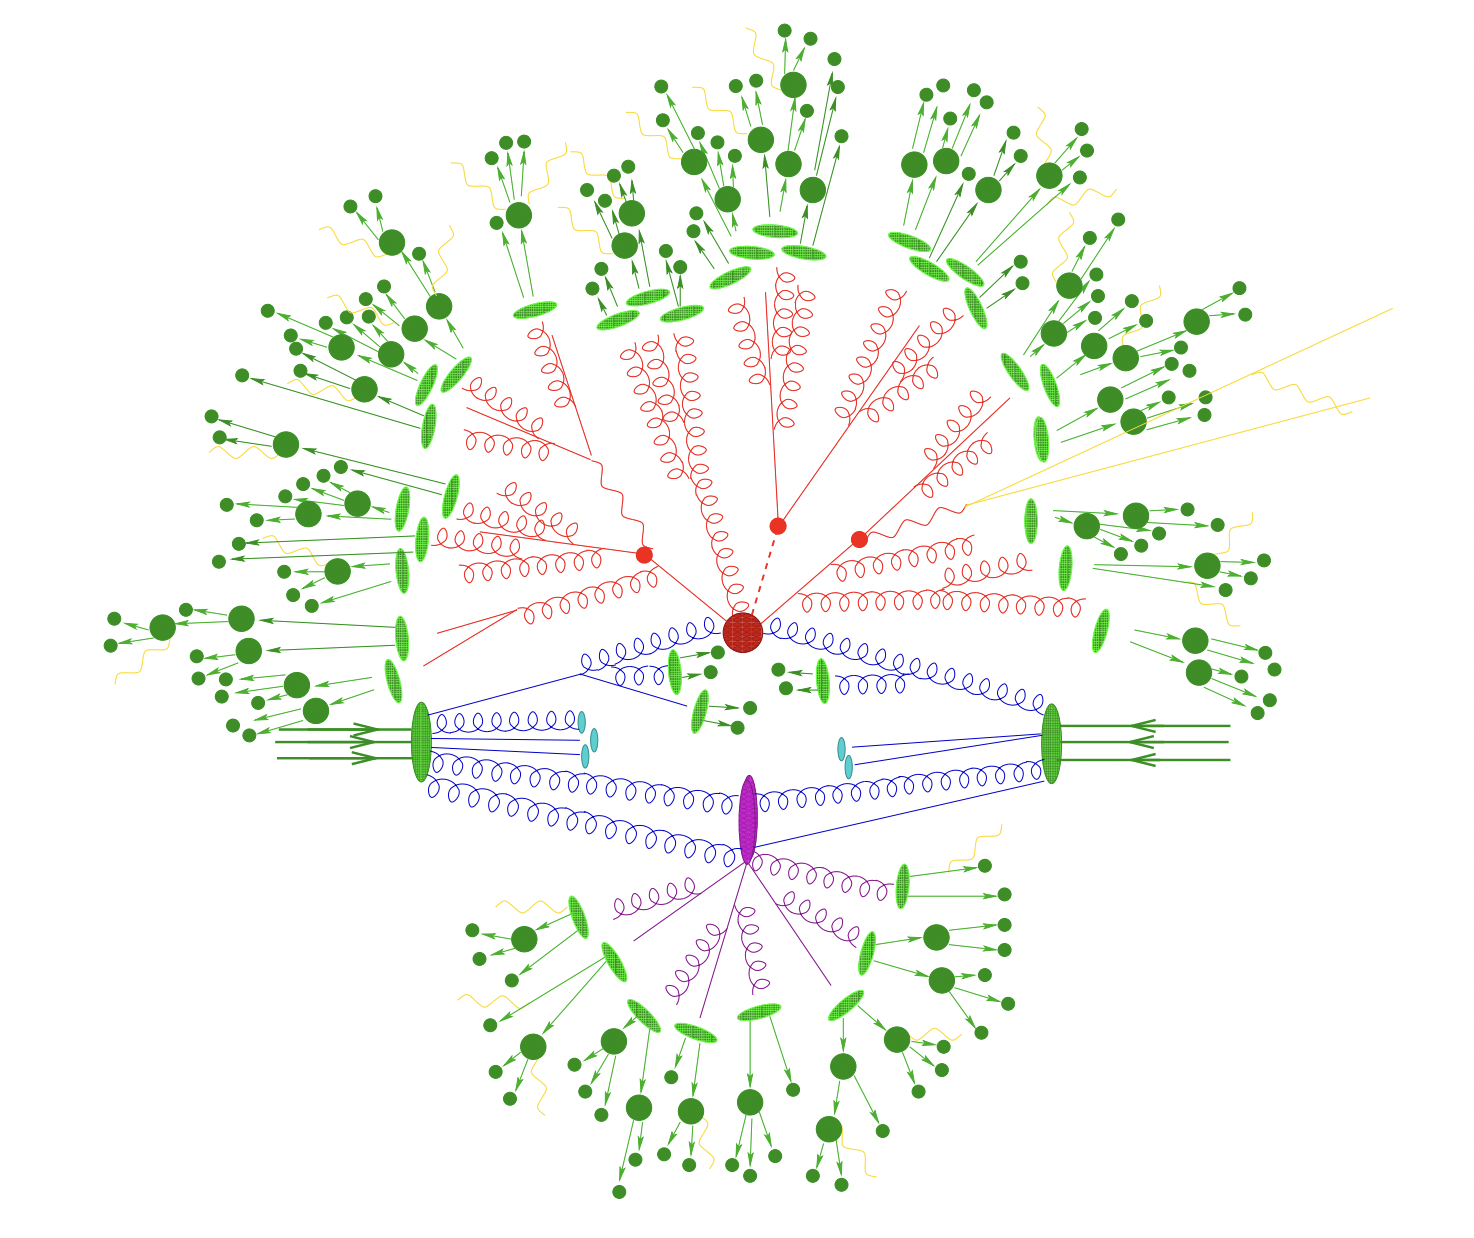
\includegraphics[width=0.7\textwidth]{figures/parton-shower}
		 }
\caption{\label{fig:parton-shower} Schematic diagram of the Monte Carlo simulation of a hadron-hadron collision. The 
incoming hadrons are the green blobs with the arrows on the left and right, with the red blob in the center 
representing the hard scatter event, and the purple representing a secondary hard scatter. Radiation from 
both incoming and outgoing particles is shown, and the light green blobs represent hadronization, with the outermost 
dark green circles corresponding to the final state hadrons. Yellow lines are radiated photons. ~\cite{parton-shower}}
\end{figure}

\FloatBarrier
\section{Detector Simulation}
Event generation provides a full and exact description of the particle content of a given collider event. 
This description is useful, but is an artifact of the simulation -- for real physics events, we must rely on 
the information collected by sophisticated detectors (Chapter \ref{chap:experiment}) to make statements about the 
physics content of collider events. The simulation of how particles interact with the physical detector and of
the corresponding information that is collected is therefore a necessary step of physics simulation at the 
LHC. The design and components of the ATLAS detector are described in Chapter \ref{chap:experiment}. 
Simulation of this detector quickly becomes complicated -- there are a variety of different materials and sub-detectors, each with particular configurations and resolutions. Interactions of particles with the detector materials can cause showering, and such showers must be simulated and characterized. 

In ATLAS, the \GEANT~\cite{GEANT4} simulation toolkit is used for detailed simulation of the ATLAS detector, often 
referred to as \emph{full simulation}. The method can be thought of as proceeding step by step as a particle moves 
through the detector, simulating the interaction of the material at each stage, and following each branch of each resulting 
shower with a similarly detailed step by step simulation. 

This type of simulation is very computationally intensive, especially in the calorimeter, which has a high density of 
material, leading to an extremely large set of material interactions to simulate. There is correspondingly a large 
effort within ATLAS to develop techniques to decrease the computational load -- these techniques will be of increasing 
importance for Run 3 and the HL-LHC, which will have increased computational need due to the high complexity and large 
volume of collected physics events, along with the corresponding set of simulated physics events~\cite{HLLHC-compute}. 
The divergence of the baseline computing model from the projected computing budget is shown in Figure \ref{fig:budget-plot}.

\begin{figure}[ht]
\centering
\subfloat{
		  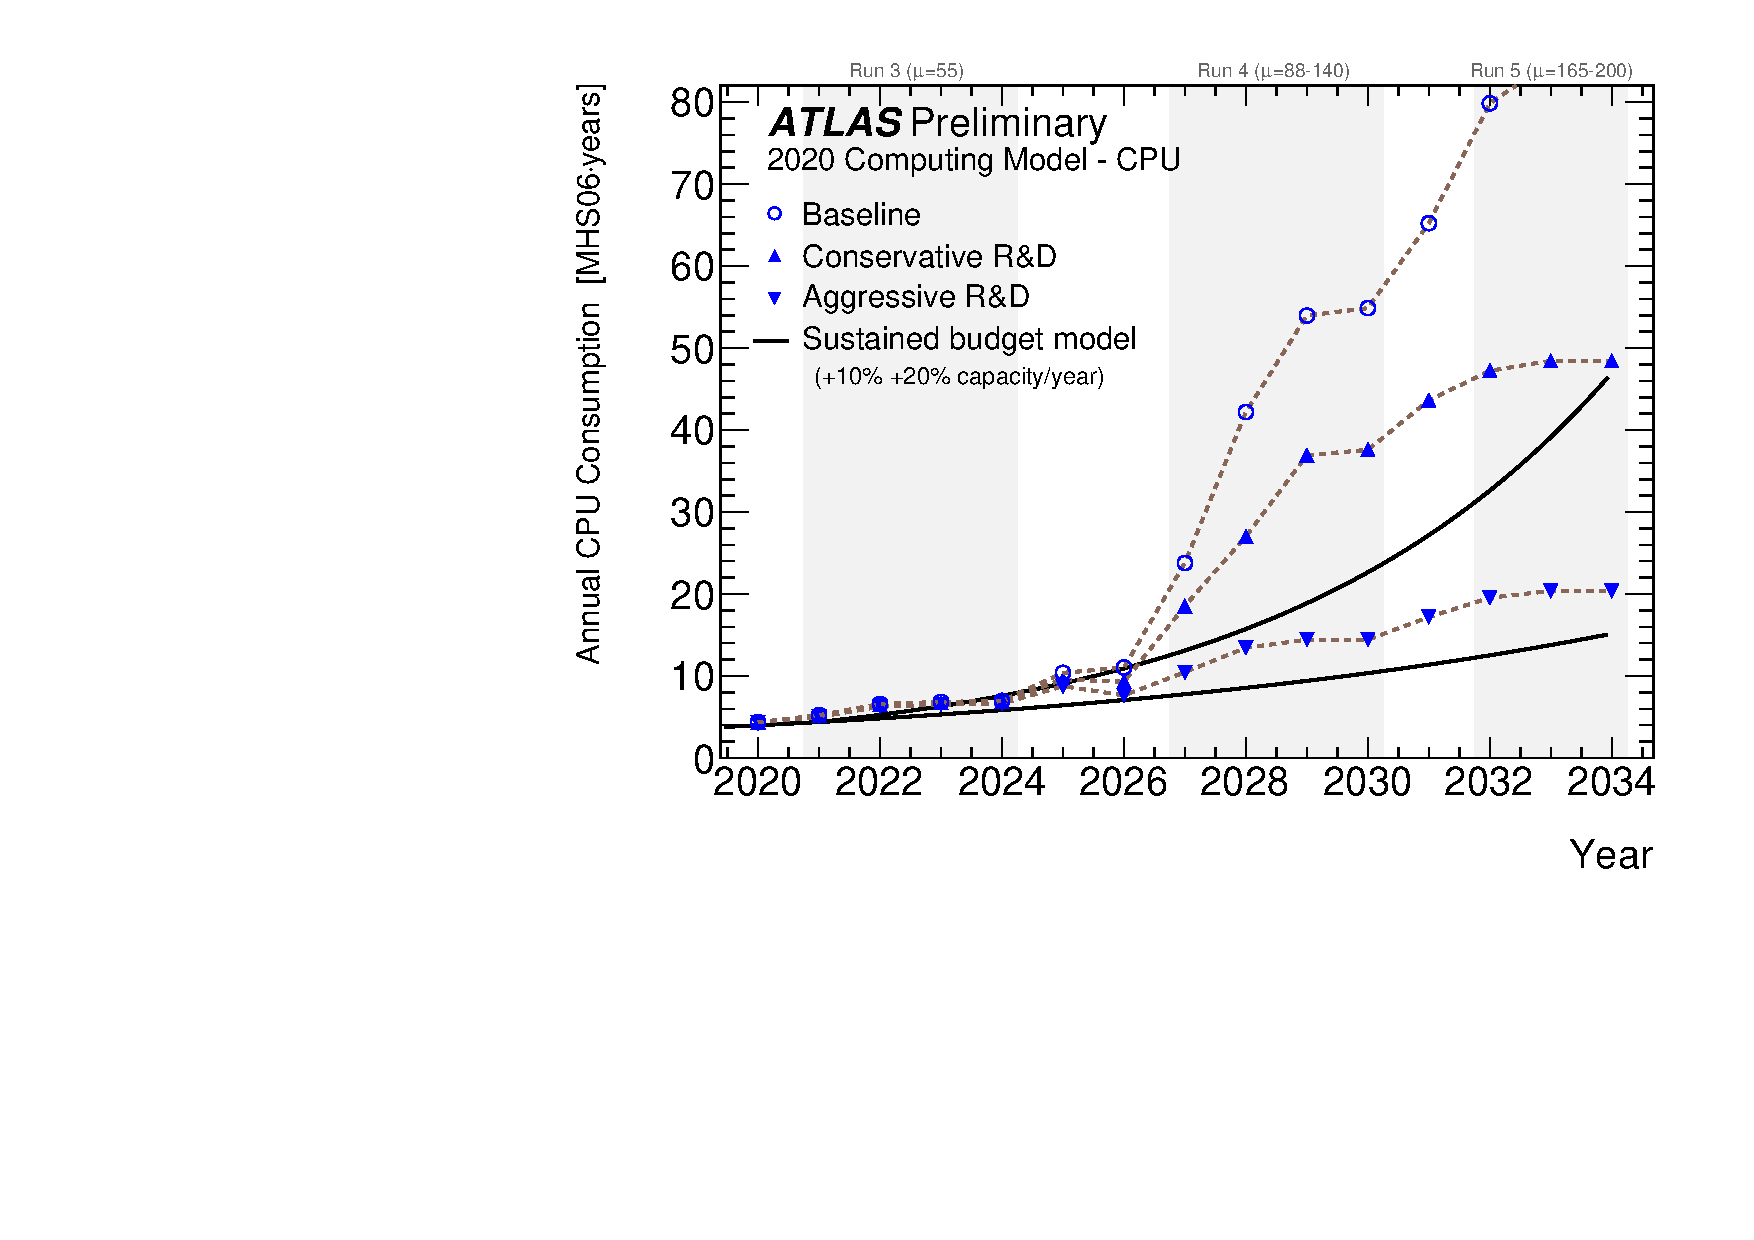
\includegraphics[width=0.7\textwidth]{figures/cpuHLLHC-ATLAS.pdf}
		 }
\caption{\label{fig:budget-plot} The projected ATLAS computational requirements for Run 3 and the HL-LHC 
relative to the projected computing budget. Aggressive R\&D is required to keep resources within 
budget~\cite{computing-budget}. $y$-axis units are MHS06 $\cdot$ years, where HS06 is a high energy 
physics specific CPU performance benchmark~\cite{HS06}.}
\end{figure}

The fast simulation used for this thesis, AtlFast-II~\cite{SOFT-2010-01}, is one such technique, which uses
a parametrized simulation of the calorimeter, called FastCaloSim, in conjunction with full simulation of the 
inner detector, to achieve an order of magnitude speed up in simulation time. This parametrized simulation uses 
a simplified detector geometry, in conjunction with a simulation of particle shower development based on statistical 
sampling of distributions from fully simulated events, to massively speed up simulation time and computational load.

Such a speed up comes at a bit of a cost in performance. In particular, the modeling of jet substructure (see Chapter 
\ref{chap:reconstruction}) historically has been an issue for FastCaloSim. The ATLAS authorship qualification work 
supporting this thesis is an effort to improve such modeling, and is part of a suite of updates being considered for 
a new fast simulation targeting Run 3. This work is briefly described in the following.

\FloatBarrier
\section{Correlated Fluctuations in FastCaloSim}
\label{shapepara}
A variety of developments have been made to FastCaloSim, improving on the version used 
for AtlFast-II. This new fast calorimeter simulation~\cite{ATL-SOFT-PUB-2018-002} is largely 
based on two components: one which describes the \emph{total energy} deposited in each calorimeter layer as a 
shower moves from the interaction point outward, and one which describes the \emph{shape}, i.e., the 
pattern of energy deposits, of a shower in each respective calorimeter layer. Both methods are 
parametrizations of the full simulation, and therefore are considered to be performing well if 
they are able to reproduce corresponding full simulation distributions. Of course, directly sampling 
from a library of showers would identically reproduce such distributions -- however a statistical 
sampling of various shower \emph{properties} provides much more generality in the simulation.

For the simulation of total energy in each given layer, the primary challenge is that such energy deposits are highly correlated. The new FastCaloSim thus relies on a technique called Principal Component Analysis (PCA)~\cite{TPrincipal} to de-correlate the layers, aiding parametrization.

The PCA chain transforms $N$ energy inputs into $N$ Gaussians and projects these Gaussians onto the eigenvectors of the corresponding covariance matrix. This results in $N$ de-correlated components, as the eigenvectors are orthogonal. The component of the PCA decomposition with the largest corresponding eigenvalue is then used to define bins, in which showers demonstrate similar patterns of energy deposition across the calorimeter layers. To further de-correlate the inputs, the PCA chain is repeated on the showers within each such bin. This full process is reversed for the particle simulation. A full description of the method can be found in \cite{ATL-SOFT-PUB-2018-002}.

Modeling of the lateral shower shape makes use of 2D histograms filled with \GEANT hit energies in each layer and PCA bin.
Binned in polar $\alpha-R$ coordinates in a local plane tangential to the surface of the calorimeter system, these histograms 
represent the spatial distribution of energy deposits for a given particle shower. Such histograms are constructed for a 
number of \GEANT events, and the histograms for each event are normalized to total energy deposited in the given layer. The 
average of these histograms is then taken (what is called here the ``average shape'').

In simulation, these average shape histograms are used as probability distributions, from which a finite number of equal 
energy hits are drawn. This finite drawing of hits induces a statistical fluctuation about the average shape which is tuned 
to match the expected calorimeter sampling uncertainty. An example such average shape is shown in Figure \ref{fig:photon-ave-shape}.
\begin{figure}[ht!]
\centering
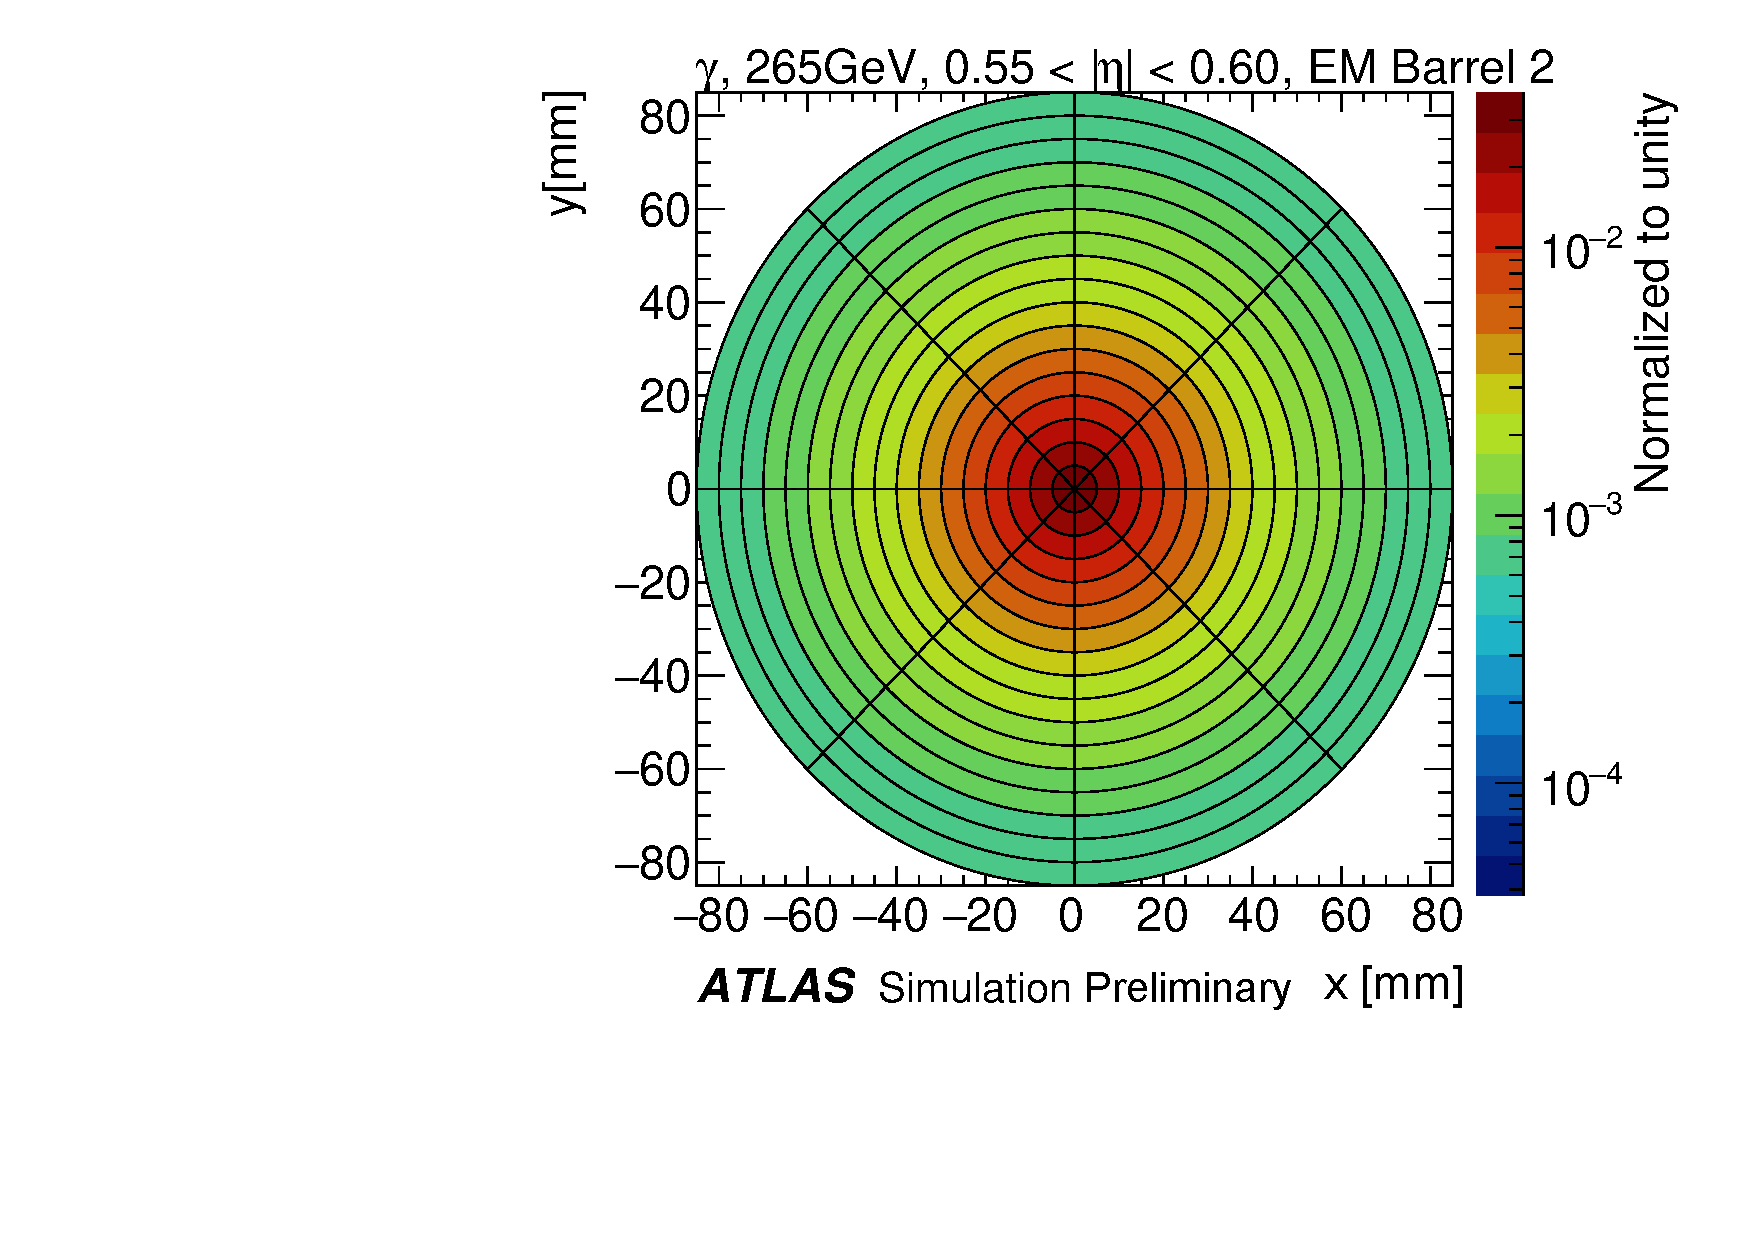
\includegraphics[width=0.6\textwidth]{figures/photon-ave-shape.pdf}
\caption{Example average lateral shower shape for a \SI{265}{\GeV} photon in the range $0.55 < |\eta| < 0.60$ in the second layer of the EM barrel. The binning shown here is in polar $\alpha-R$ coordinates in a local plane 
tangential to the surface of the calorimeter system. Such a histogram is used as a probability distribution, from 
which a finite number of ``hits'' are drawn ~\cite{ATL-SOFT-PUB-2018-002}.}
\label{fig:photon-ave-shape} 
\end{figure}

As an example, the intrinsic resolution of the ATLAS Liquid Argon calorimeter has a sampling term of 
$\sigma_{\text{samp}} \approx 10\%/\sqrt{E}$ \cite{SamplingCalo}. The number of hits to be drawn for each layer, 
$N_{\text{hits}}^{\text{layer}}$, is thus taken from a Poisson distribution with mean $1/\sigma_{\text{samp}}^2$, where the 
energy assigned to each hit is then just $E_{\text{hit}} = \frac{E_{\text{layer}}}{N_{\text{hits}}^{\text{layer}}}$. This 
induces a fluctuation of the order of $10\%/\sqrt{E_{\text{bin}}}$ for each bin in the average shape.

Figure \ref{fig-1} shows a comparison of energy and weta2~\cite{ATLAS-CONF-2010-077}, defined as the energy weighted lateral width of a 
shower in the second electromagnetic calorimeter layer, for 16 GeV photons simulated with the new FastCaloSim and with full 
\GEANT simulation. The agreement is quite good, with FastCaloSim matching the \GEANT mean to within 0.3 and 0.03 percent 
respectively. Similar results are seen for other photon energies and $\eta$ points.
\begin{figure}[ht!]
\centering
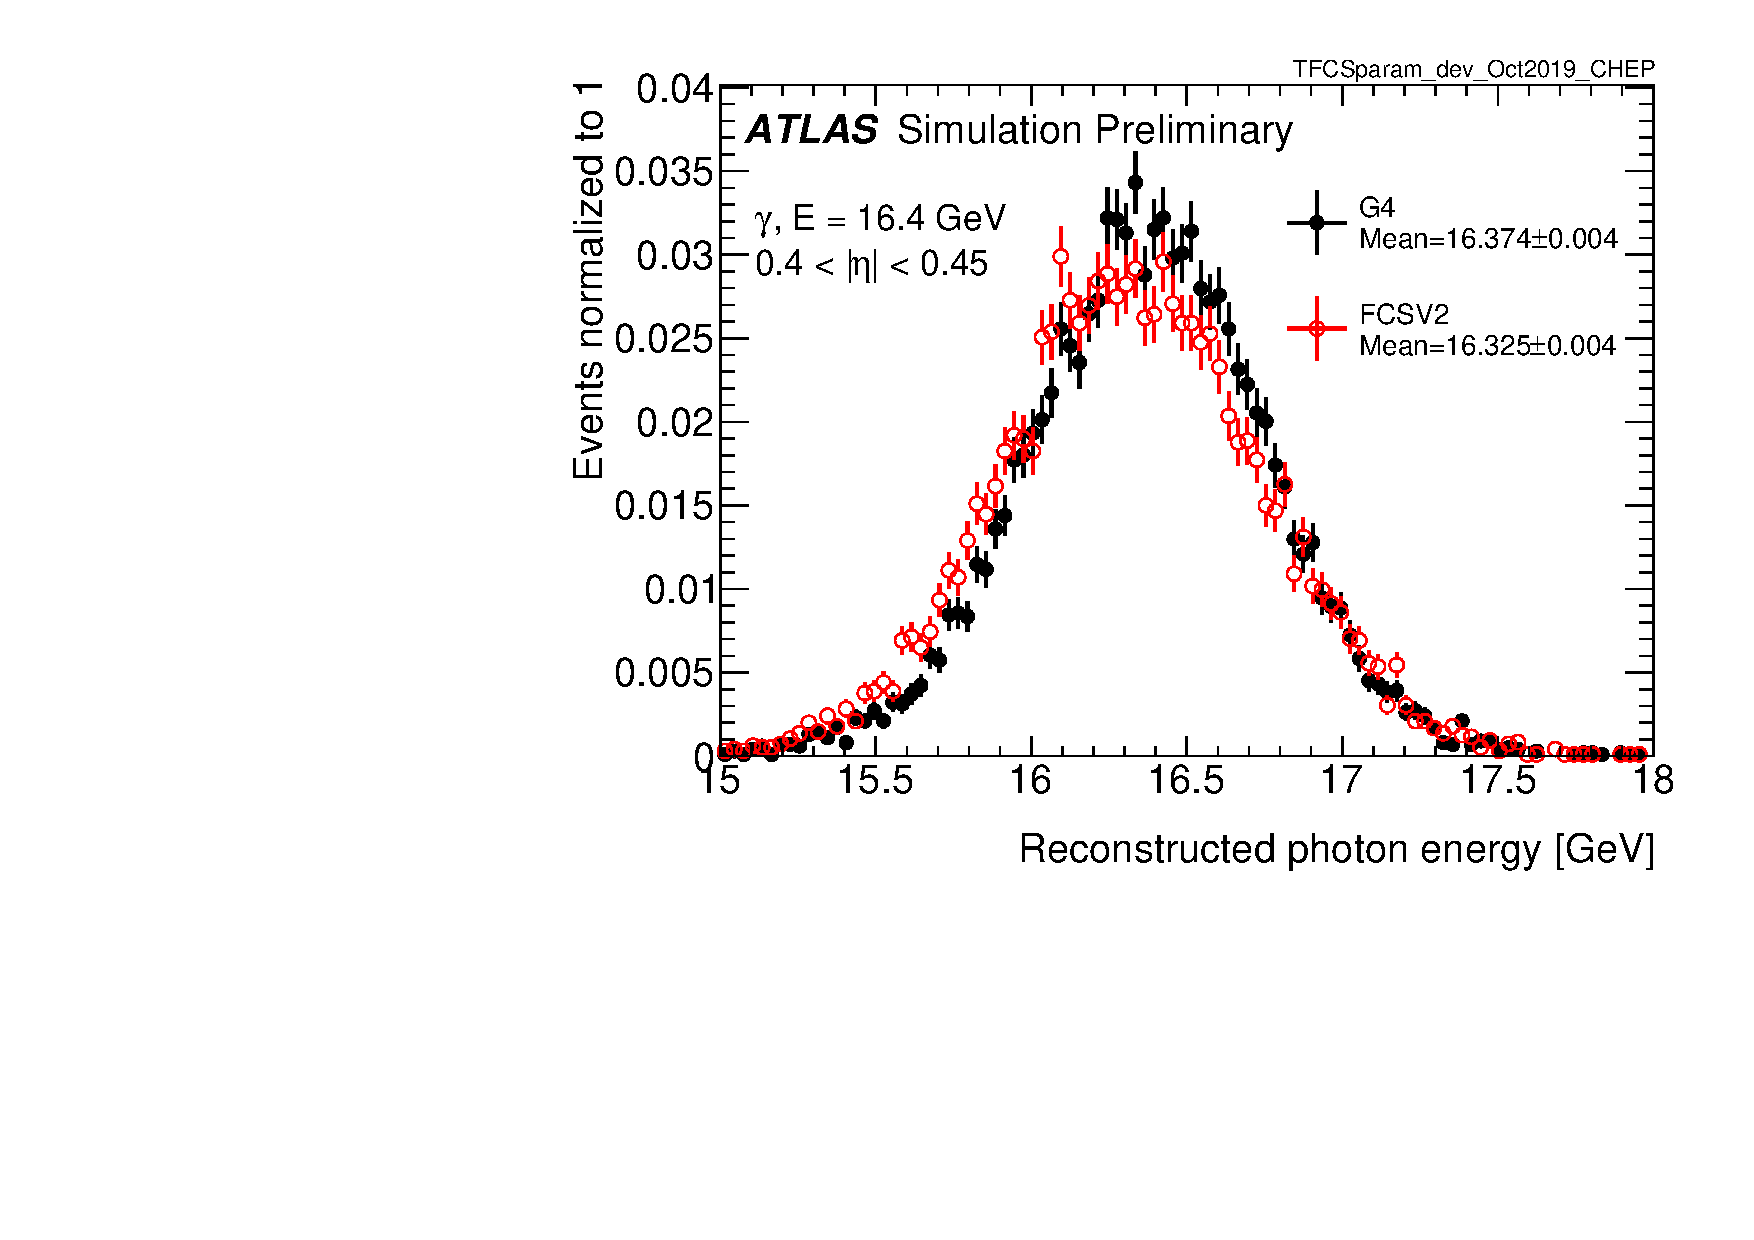
\includegraphics[width=0.48\textwidth]{figures/CHEP-photon-energy.pdf}
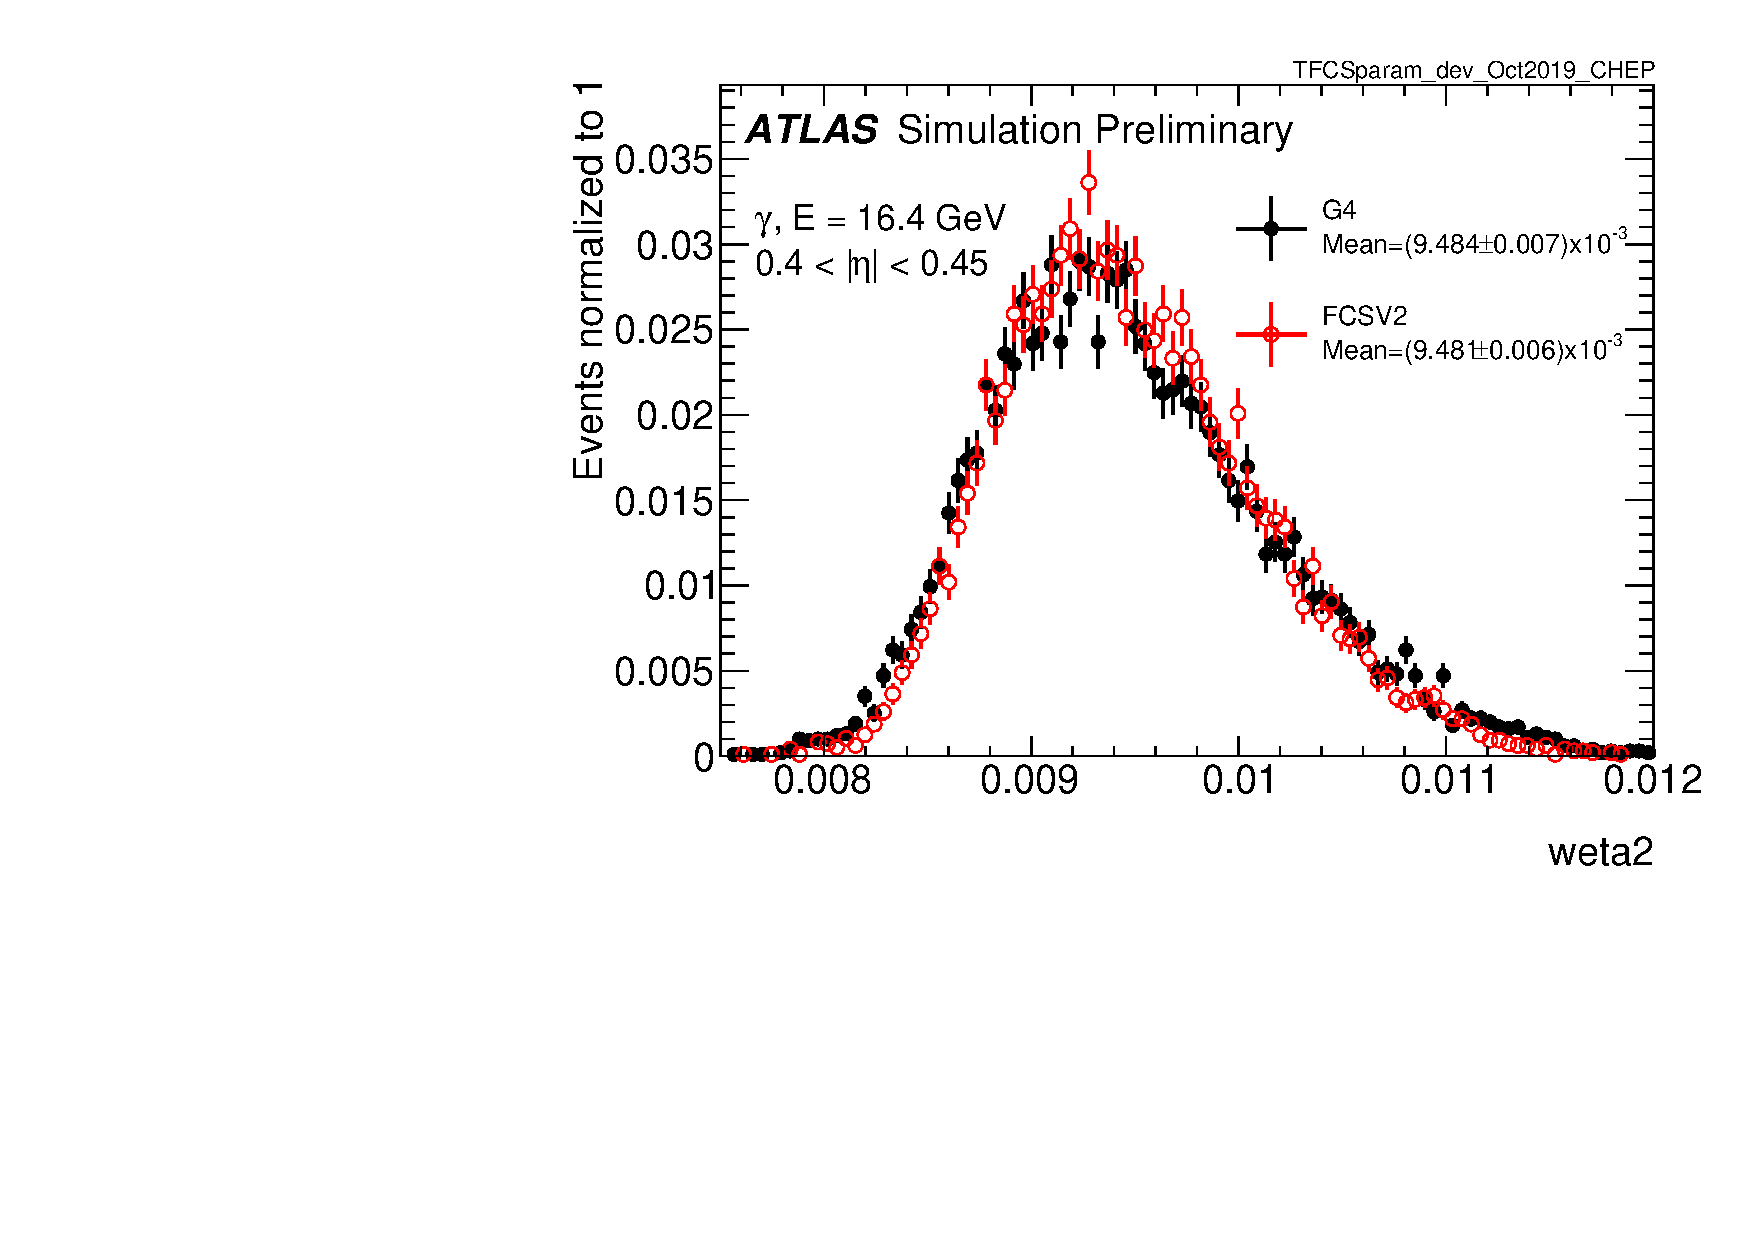
\includegraphics[width=0.48\textwidth]{figures/CHEP-photon-weta2.pdf}
\caption{Energy and variable weta2, defined as the energy weighted lateral width of a shower in the second electromagnetic calorimeter layer, for 16 GeV photons with full simulation (G4) and FastCaloSimV2 (FCSV2) \cite{ATL-SOFT-PUB-2018-002}.}
\label{fig-1} 
\end{figure}

\FloatBarrier
\subsection{Fluctuation Modeling}
\label{fluct-modeling}
Figure \ref{fig-2} shows the ratio of calorimeter cell energies for single \GEANT photon and pion events to the corresponding 
cell energies in their respective average shapes. While the photon event is quite close to the corresponding average, the 
pion event shows a deviation from the average which is much larger and has a non-trivial structure, reflecting the different 
natures of electromagnetic and hadronic showering.

While the shape parametrization described above is thus sufficient for describing electromagnetic showers, we will demonstrate below that it is not sufficient for describing hadronic showers (Figures \ref{fig-5} and \ref{fig-6}). We therefore present and validate methods to improve this hadronic shower modeling. Such methods have been presented as well in~\cite{CHEP-proceedings}.

\begin{figure}[ht!]
\centering
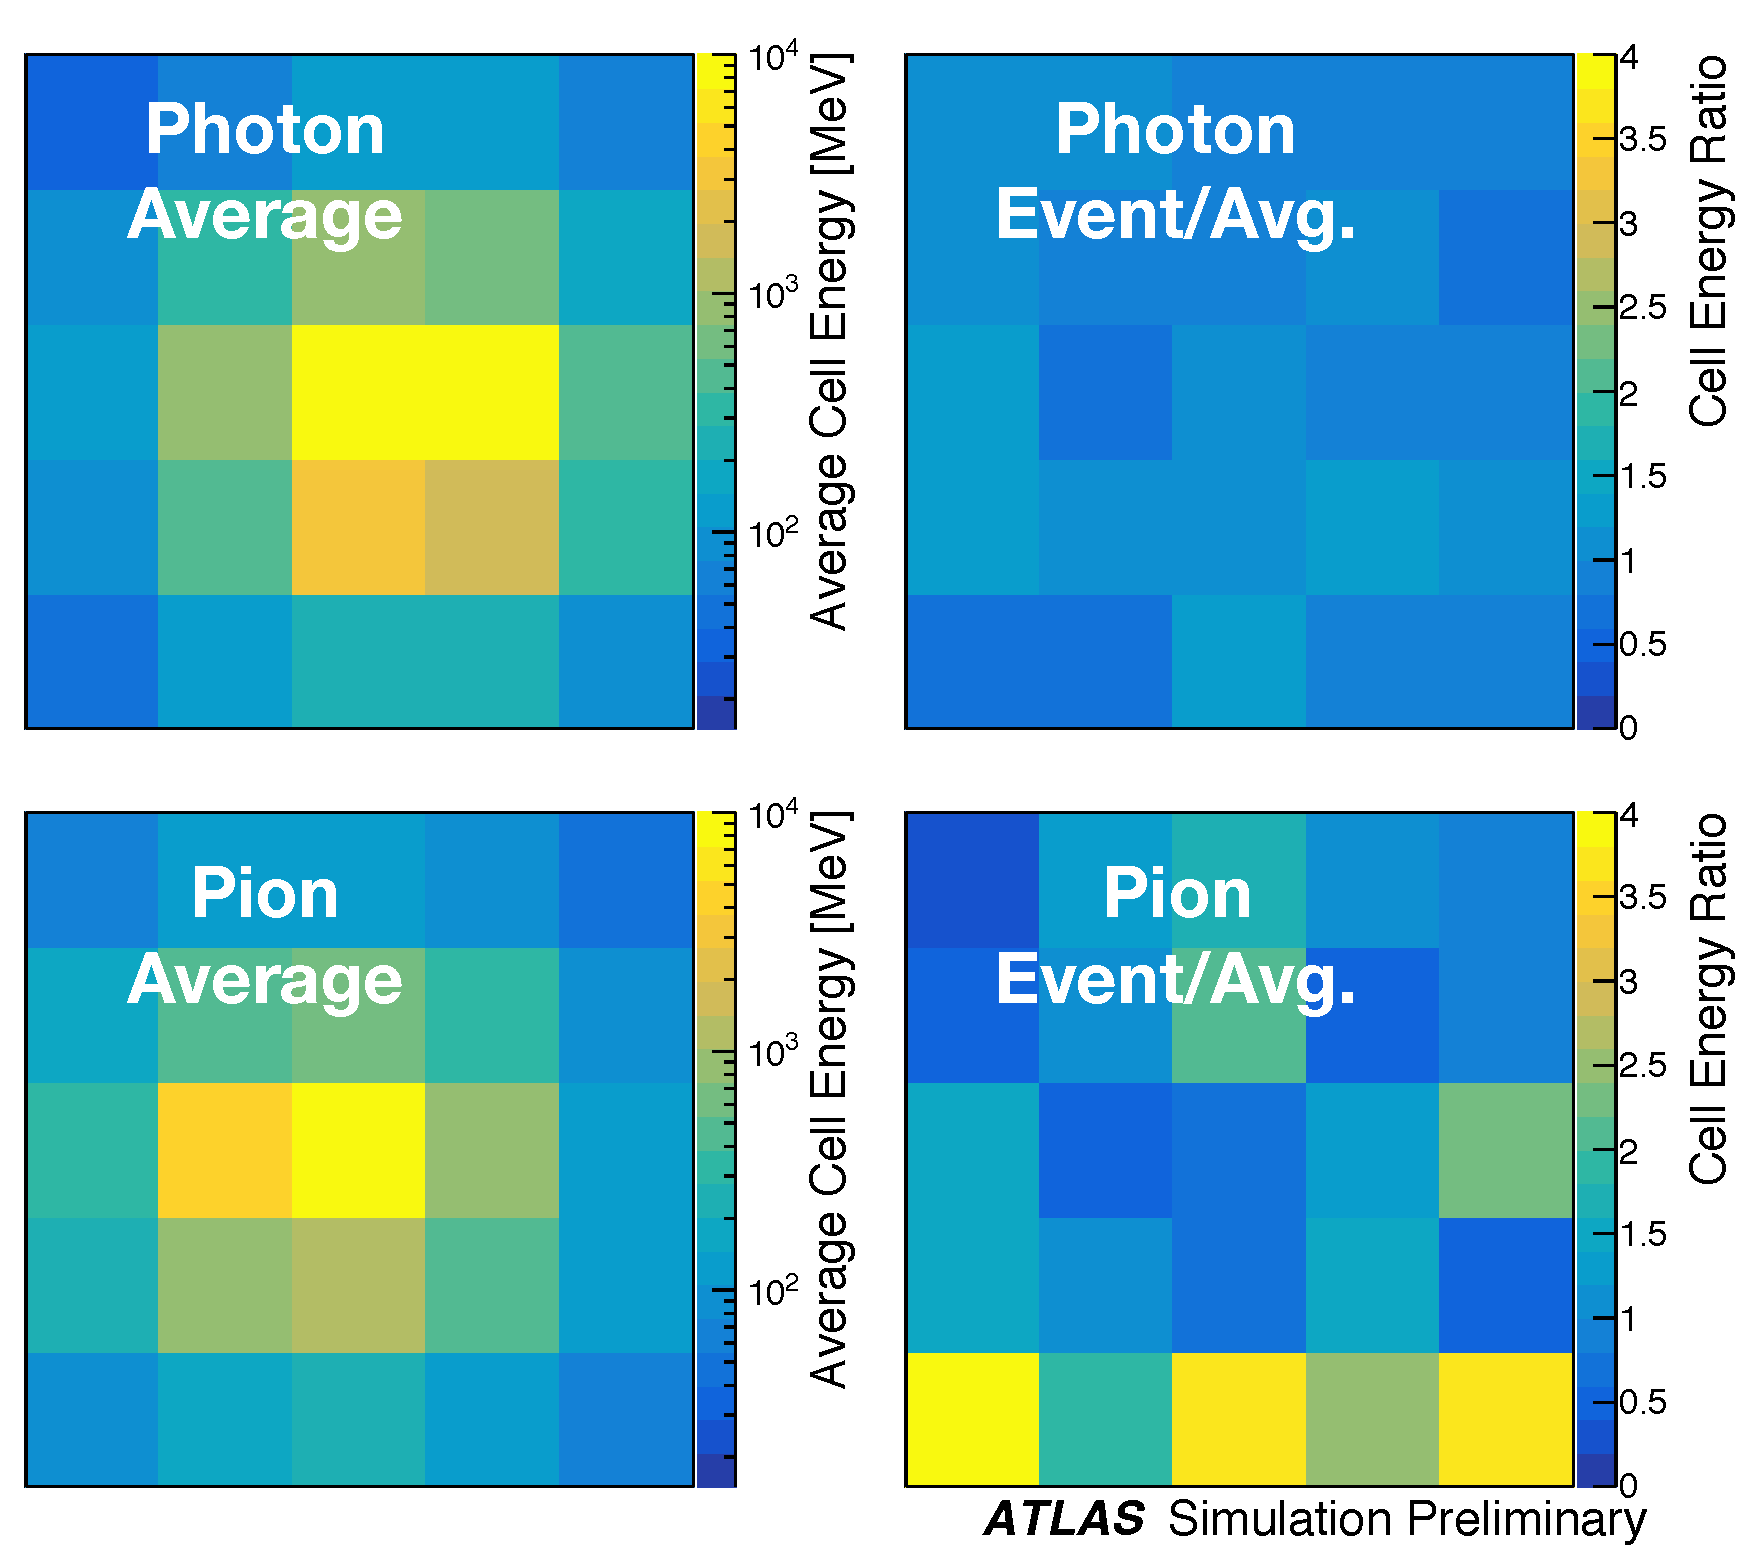
\includegraphics[width=0.7\textwidth]{figures/approved-example-pion-photon-ave-ratios-ATLASstyle.pdf}
\caption{Example of photon and pion average shapes in 5 $\times$ 5 calorimeter cells. The left column shows the average shape over a sample of 10000 events, while the right column shows the energy ratio, in each cell, of single \GEANT events with respect to this average. The photon ratios are all close to 1, while the pion ratios show significant deviation from the average.}
\label{fig-2}
\end{figure}

Two methods for modeling deviations from the average shape have been studied: 
(1) a neural network based approach using a Variational 
Autoencoder (VAE) \cite{VAE} and (2) a map through cumulative distributions to an $n$-dimensional Gaussian. 
With both methods, the shape simulation then proceeds as described in Section \ref{shapepara}, with the drawing of hits 
according to the average shape. However, these hits no longer have equal energy, but have weights applied to increase or 
decrease their energy depending on their spatial position. This application of weights is designed to mimic a realistic 
shower structure and to encode correlations between energy deposits.

Both methods are trained on ratios of energy in binned units called voxels. This voxelization is performed in the same polar 
$\alpha-R$ coordinates as the average shape, with a 5 mm core in $R$ and 20 mm binning thereafter. There are a total of 8 
$\alpha$ bins from 0 to $2\pi$ and 8 additional $R$ bins from 5 mm to 165 mm. The 5 mm core is filled with the average value 
of core voxels across the 8 $\alpha$ bins when creating the parametrization. However, during simulation, each of these 8 core 
bins is treated independently. The outputs of both methods mimic these energy ratios and are used in the shape simulation as 
the weights described above. In contrast to an approach based on, e.g., calorimeter cells, using voxels allows for 
flexibility in tuning the binning used in creating the parametrization. Further, due to their relatively large size, using 
calorimeter cells is subject to ``edge effects'', where the splitting of energy between cells has a non-trivial effect on the 
observed energy ratio. The binning used here is of the order of half of a cell size, mitigating this effect.

The Gaussian method operates by using cumulative distributions to map \GEANT energy ratios to a multidimensional Gaussian 
distribution. New events are generated by randomly sampling from this Gaussian distribution.

For the VAE method, a system of two linked neural networks is trained to generate events. The first ``encoder'' neural 
network maps input \GEANT energy ratios to a lower dimensional latent space. A second ``decoder'' neural network then samples 
from that latent space and tries to reproduce the inputs. In simulation, events are generated by taking random samples from 
the latent space and passing them through the trained decoder.

\begin{figure}[ht!]
\centering
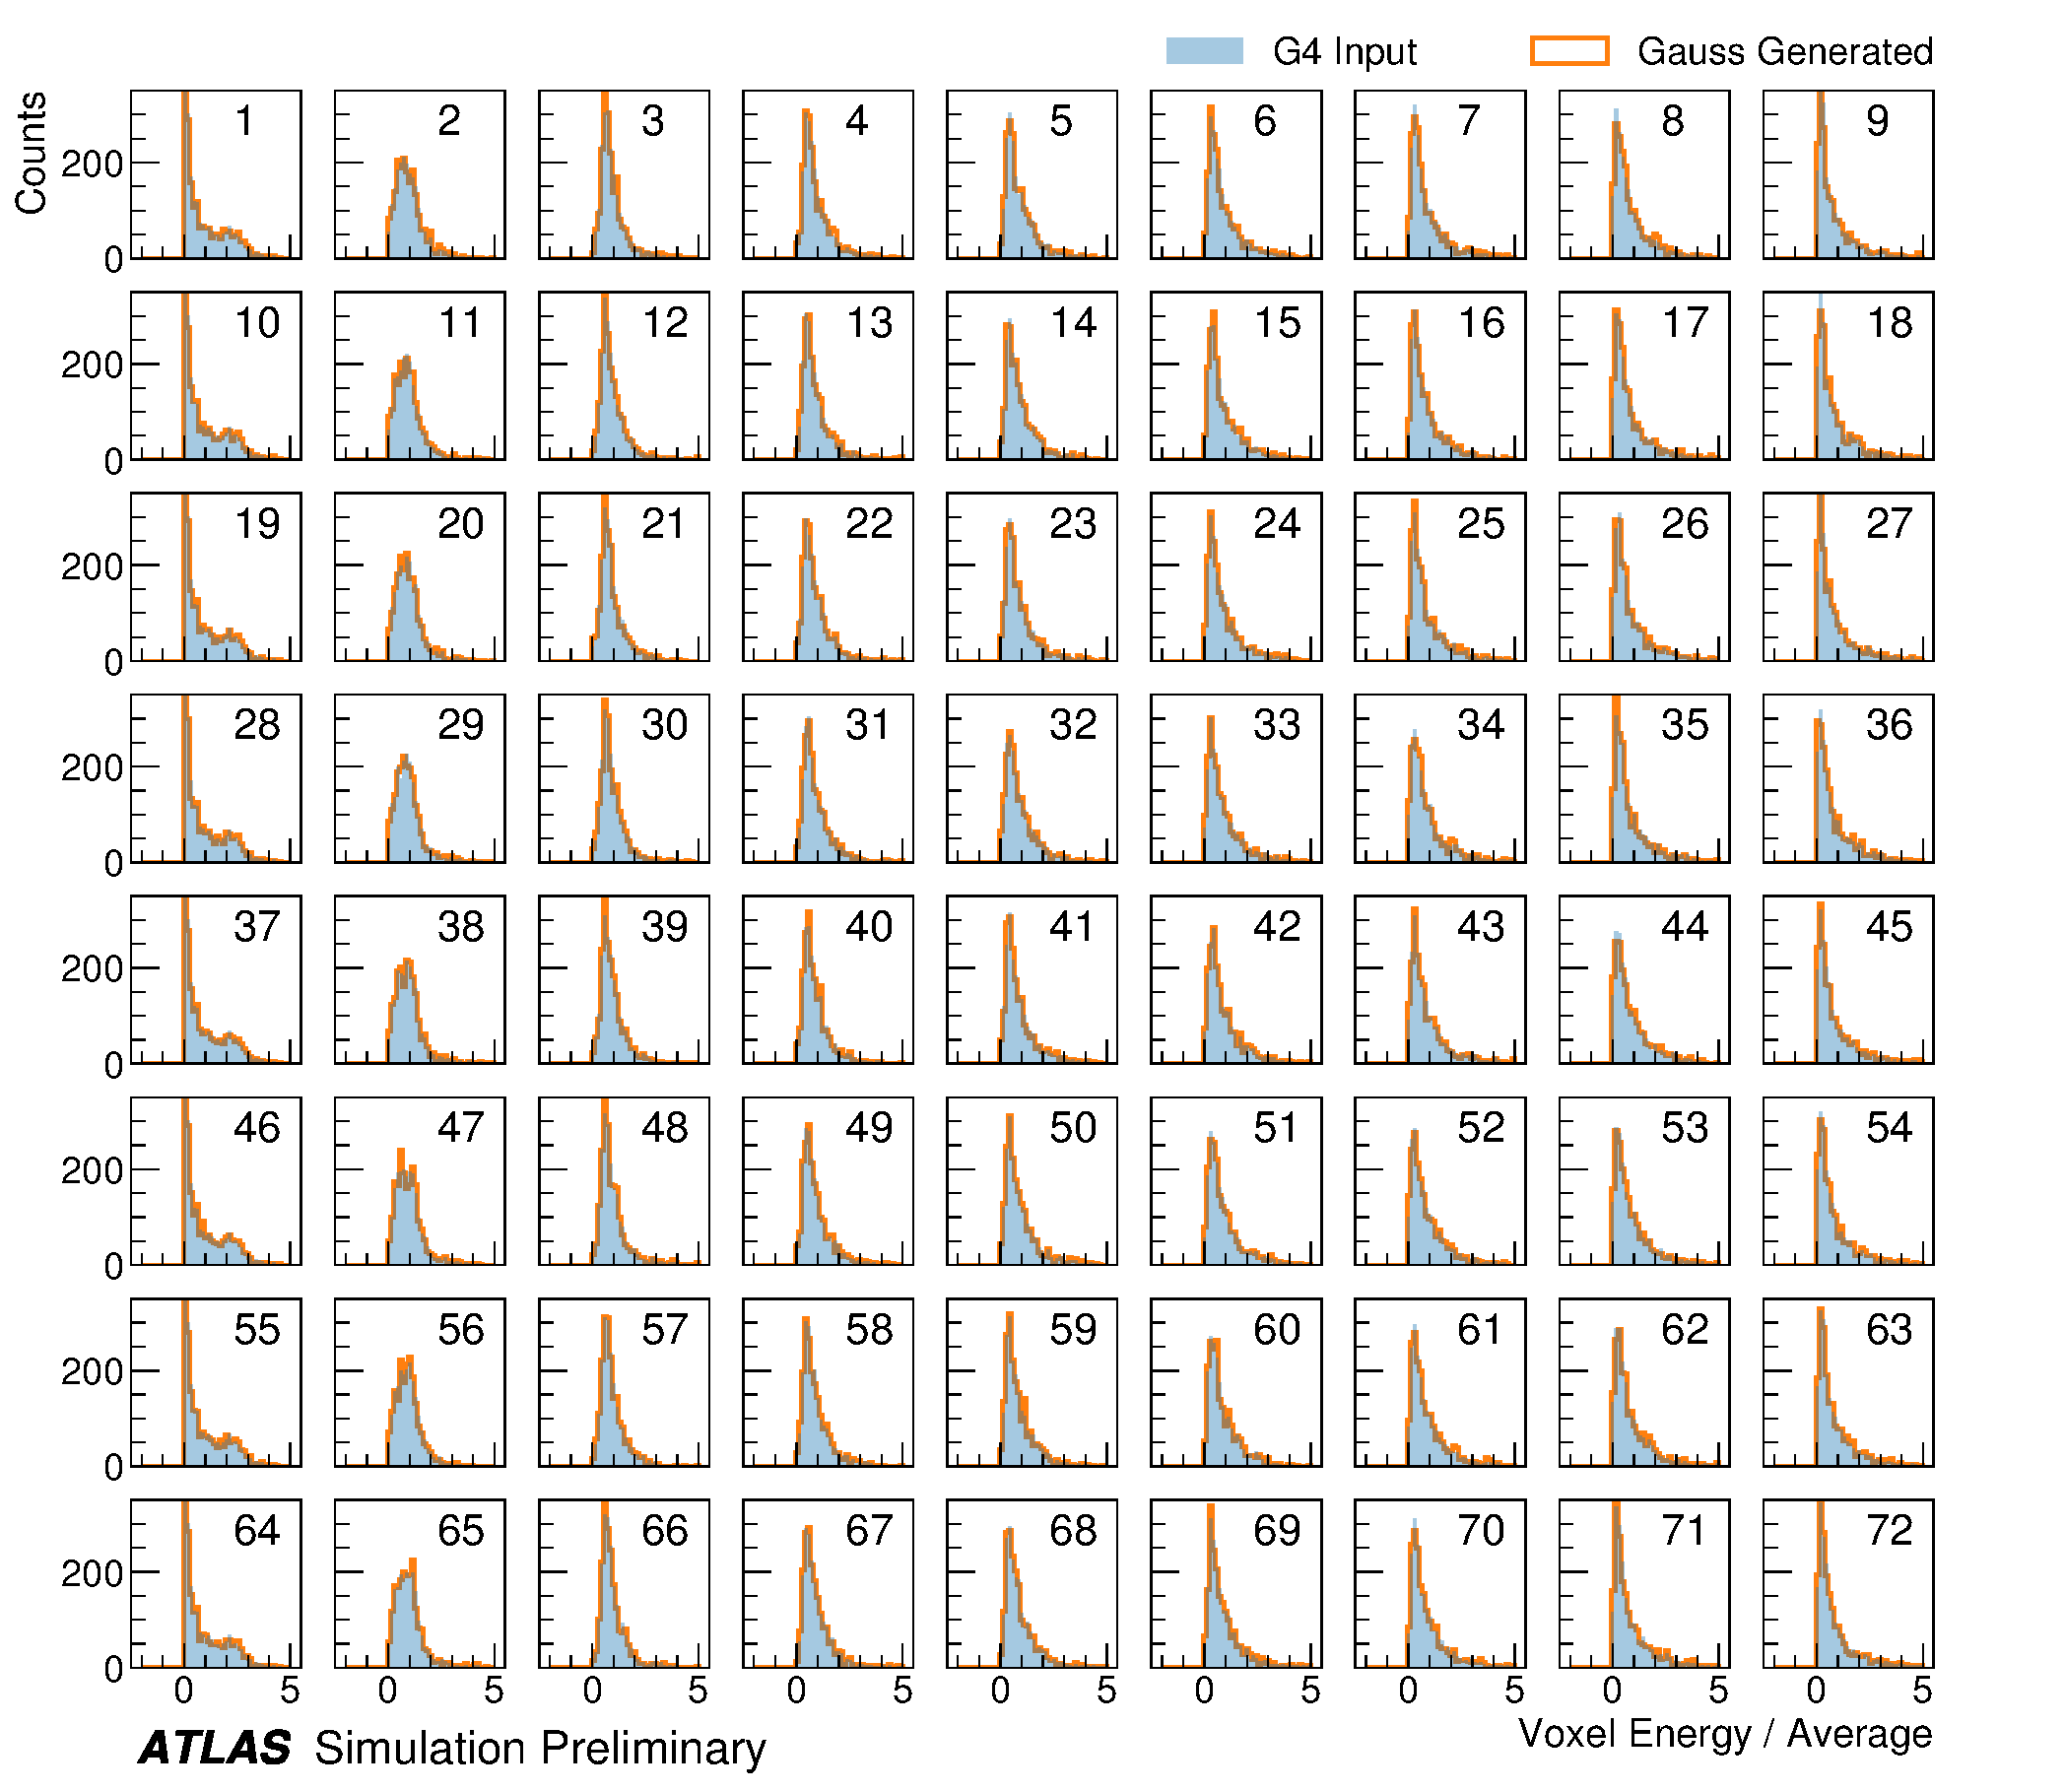
\includegraphics[width=0.7\textwidth]{figures/FCS-fig-02.pdf}
\caption{Distribution of the ratio of voxel energy in single events to the corresponding voxel energy in the average shape, with \GEANT events in blue and Gaussian model events in orange, for 65 GeV central pions in EMB2. Moving top to bottom corresponds to increasing $\alpha$, left to right corresponds to increasing $R$, with core voxels numbered 1, 10, 19, \ldots. Agreement is quite good across all voxels. Results are similar for the VAE method.}
\label{fig-3}       % Give a unique label
\end{figure}

\begin{figure}[ht!]
\centering
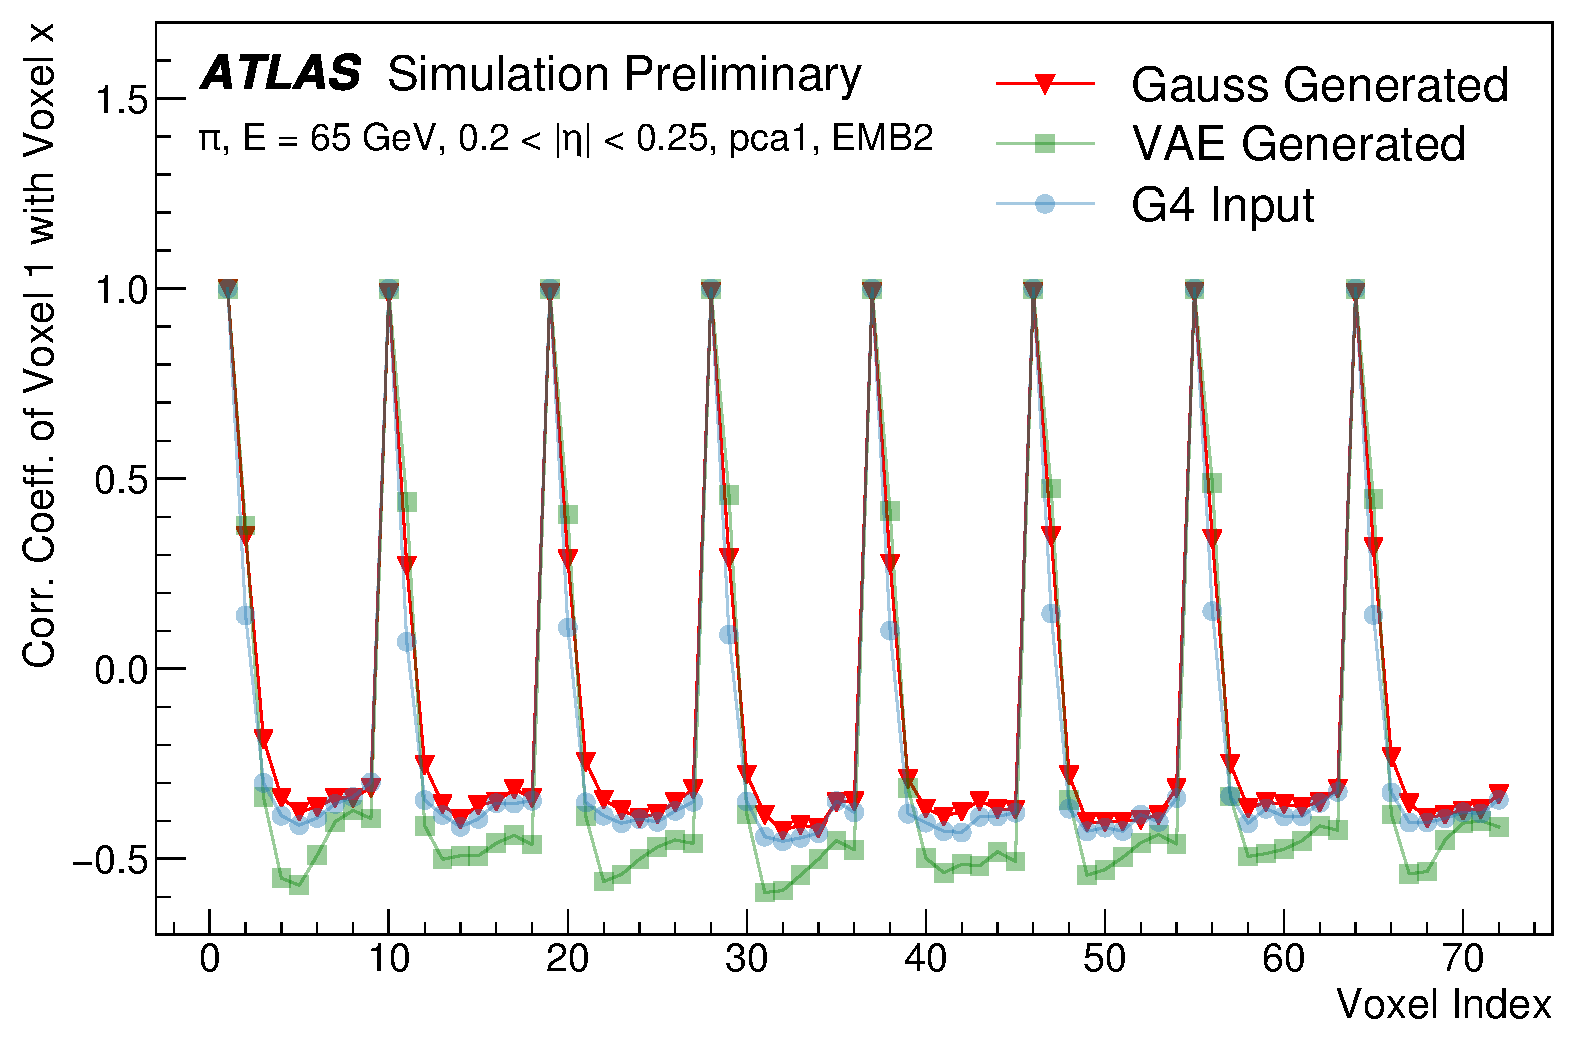
\includegraphics[width=0.7\textwidth]{figures/FCS-fig-01-new.pdf}
\caption{Correlation coefficient of ratios of voxel energy in single events to the corresponding voxel energy in the average shape, examined between the core bin from $\alpha = 0$ to $2\pi/8$ and each of the other voxels. The periodic structure represents the binning in $\alpha$, and the increasing numbers in each of these periods correspond to increasing $R$, where the eight points with correlation coefficient 1 are the eight core bins. Both the Gaussian and VAE generated toy events are able to reproduce the major correlation structures for 65 GeV central pions in EMB2.}
\label{fig-4}       % Give a unique label
\end{figure}

Figure \ref{fig-3} shows the distributions of input \GEANT and Gaussian method generated energy ratios in the grid of voxels. Figure \ref{fig-4} shows the correlation coefficient between the center voxel from $\alpha = 0$ to $2\pi/8$ for input \GEANT and the Gaussian and VAE fluctuation methods. Agreement is good throughout. 

\begin{figure}[ht!]
\centering
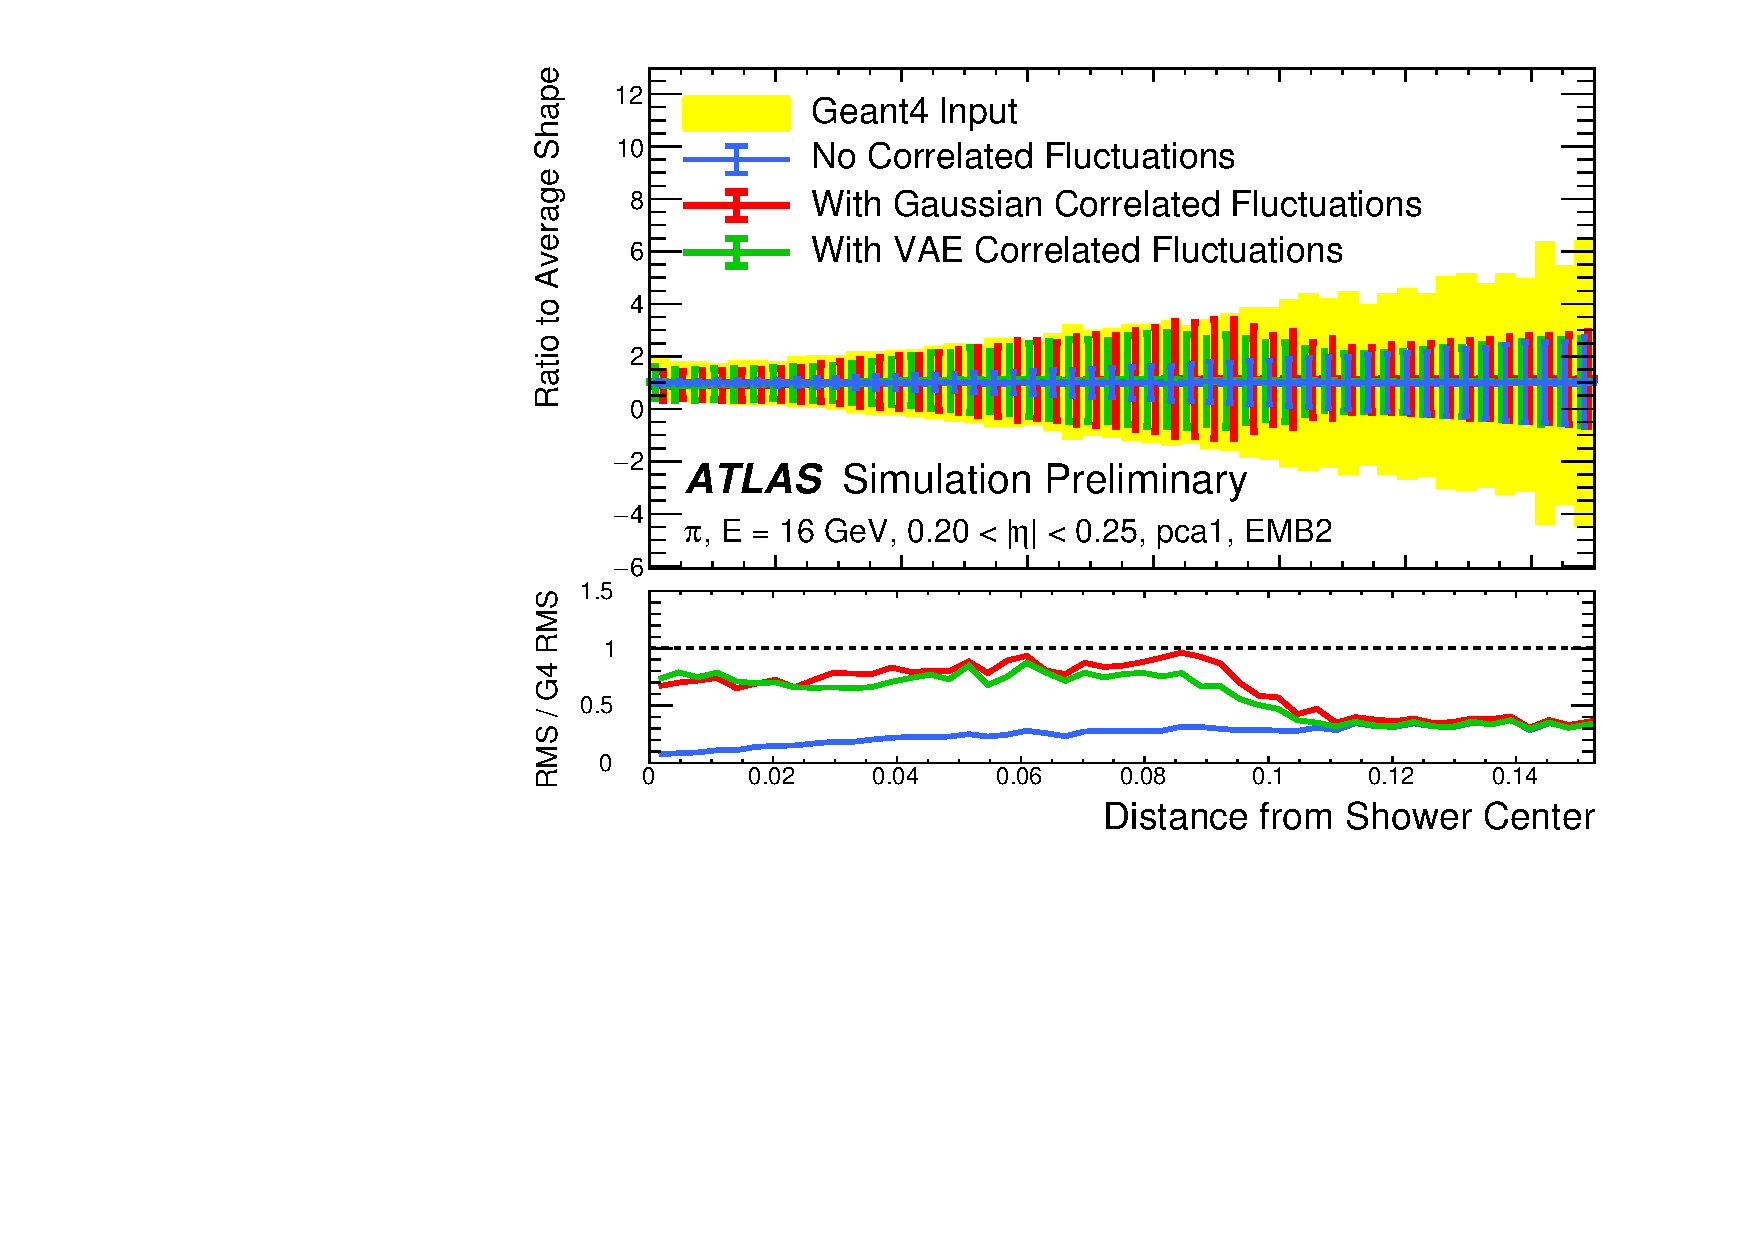
\includegraphics[width=0.48\textwidth]{figures/FCS-fig-03.pdf}
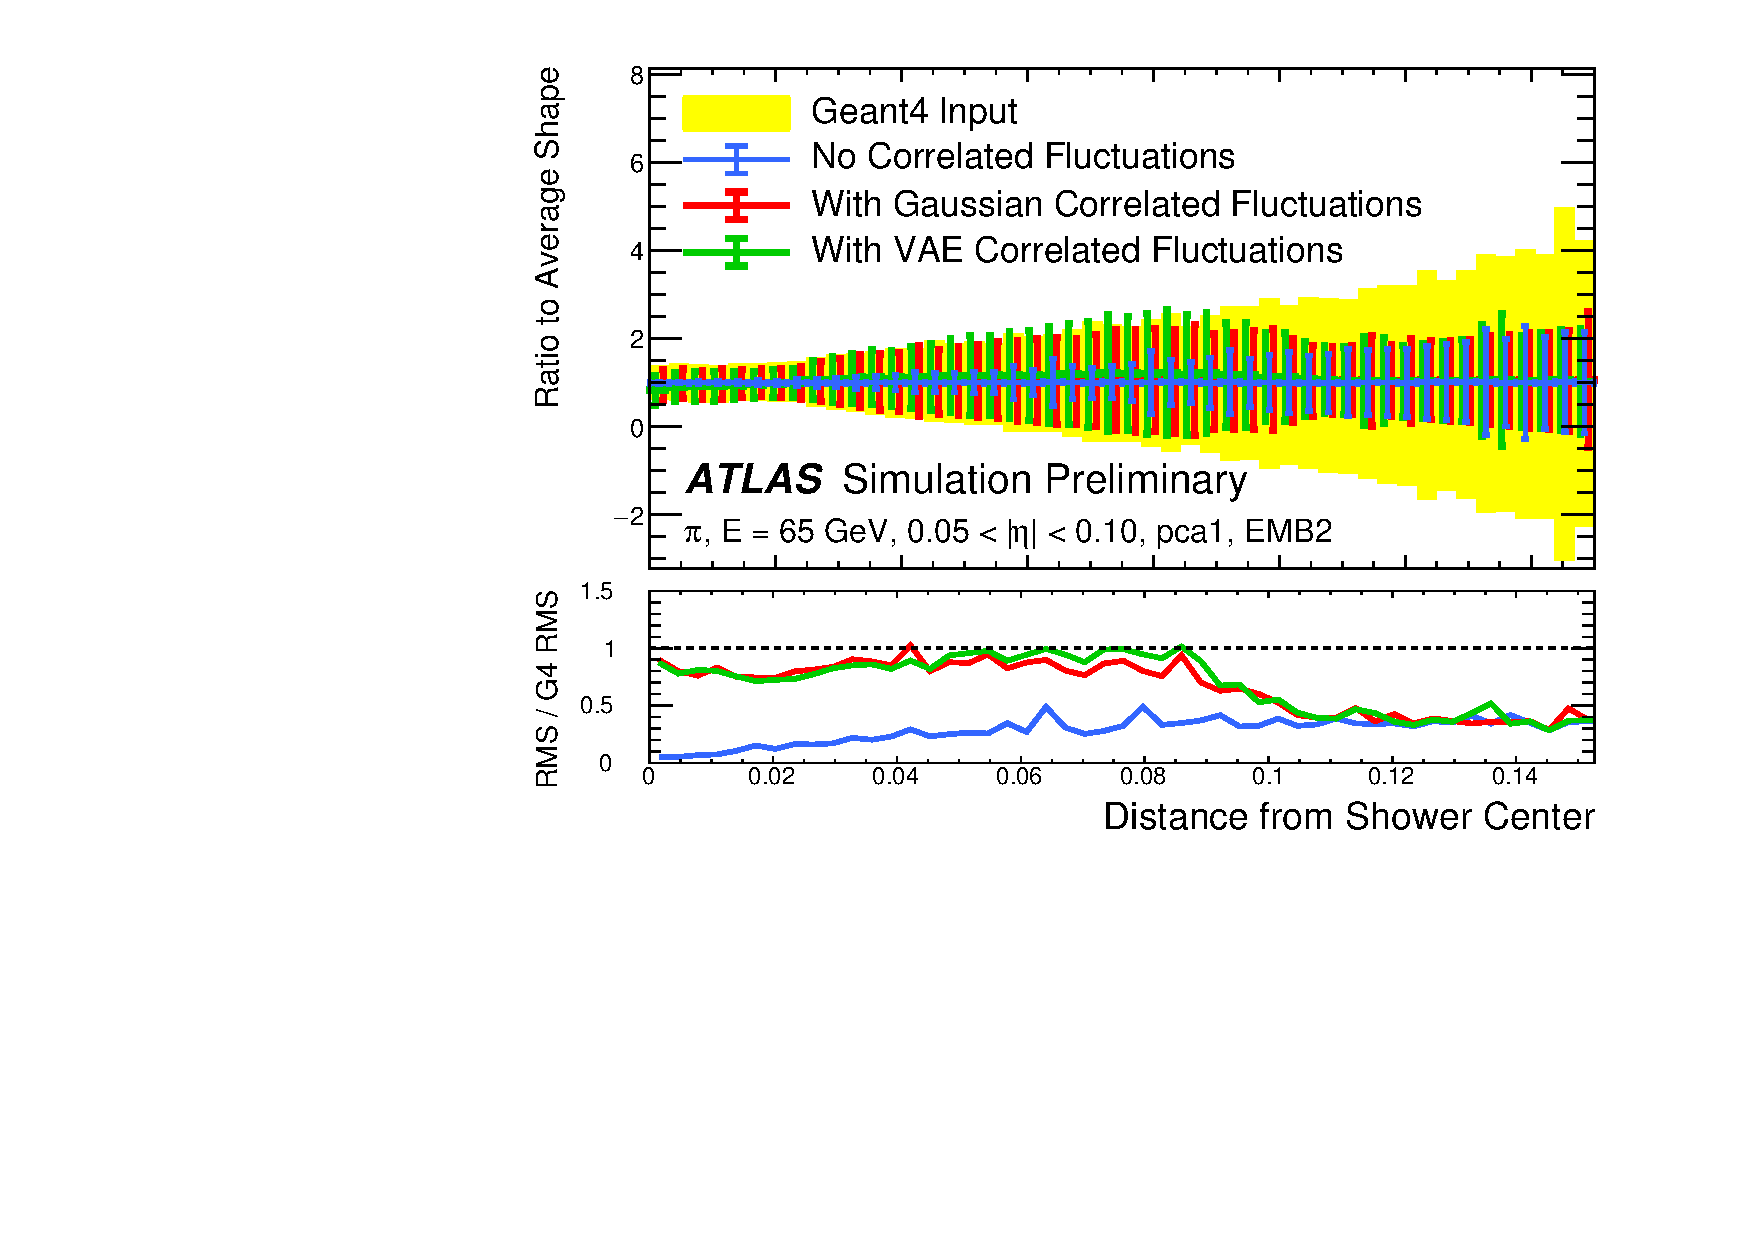
\includegraphics[width=0.48\textwidth]{figures/FCS-fig-04.pdf}
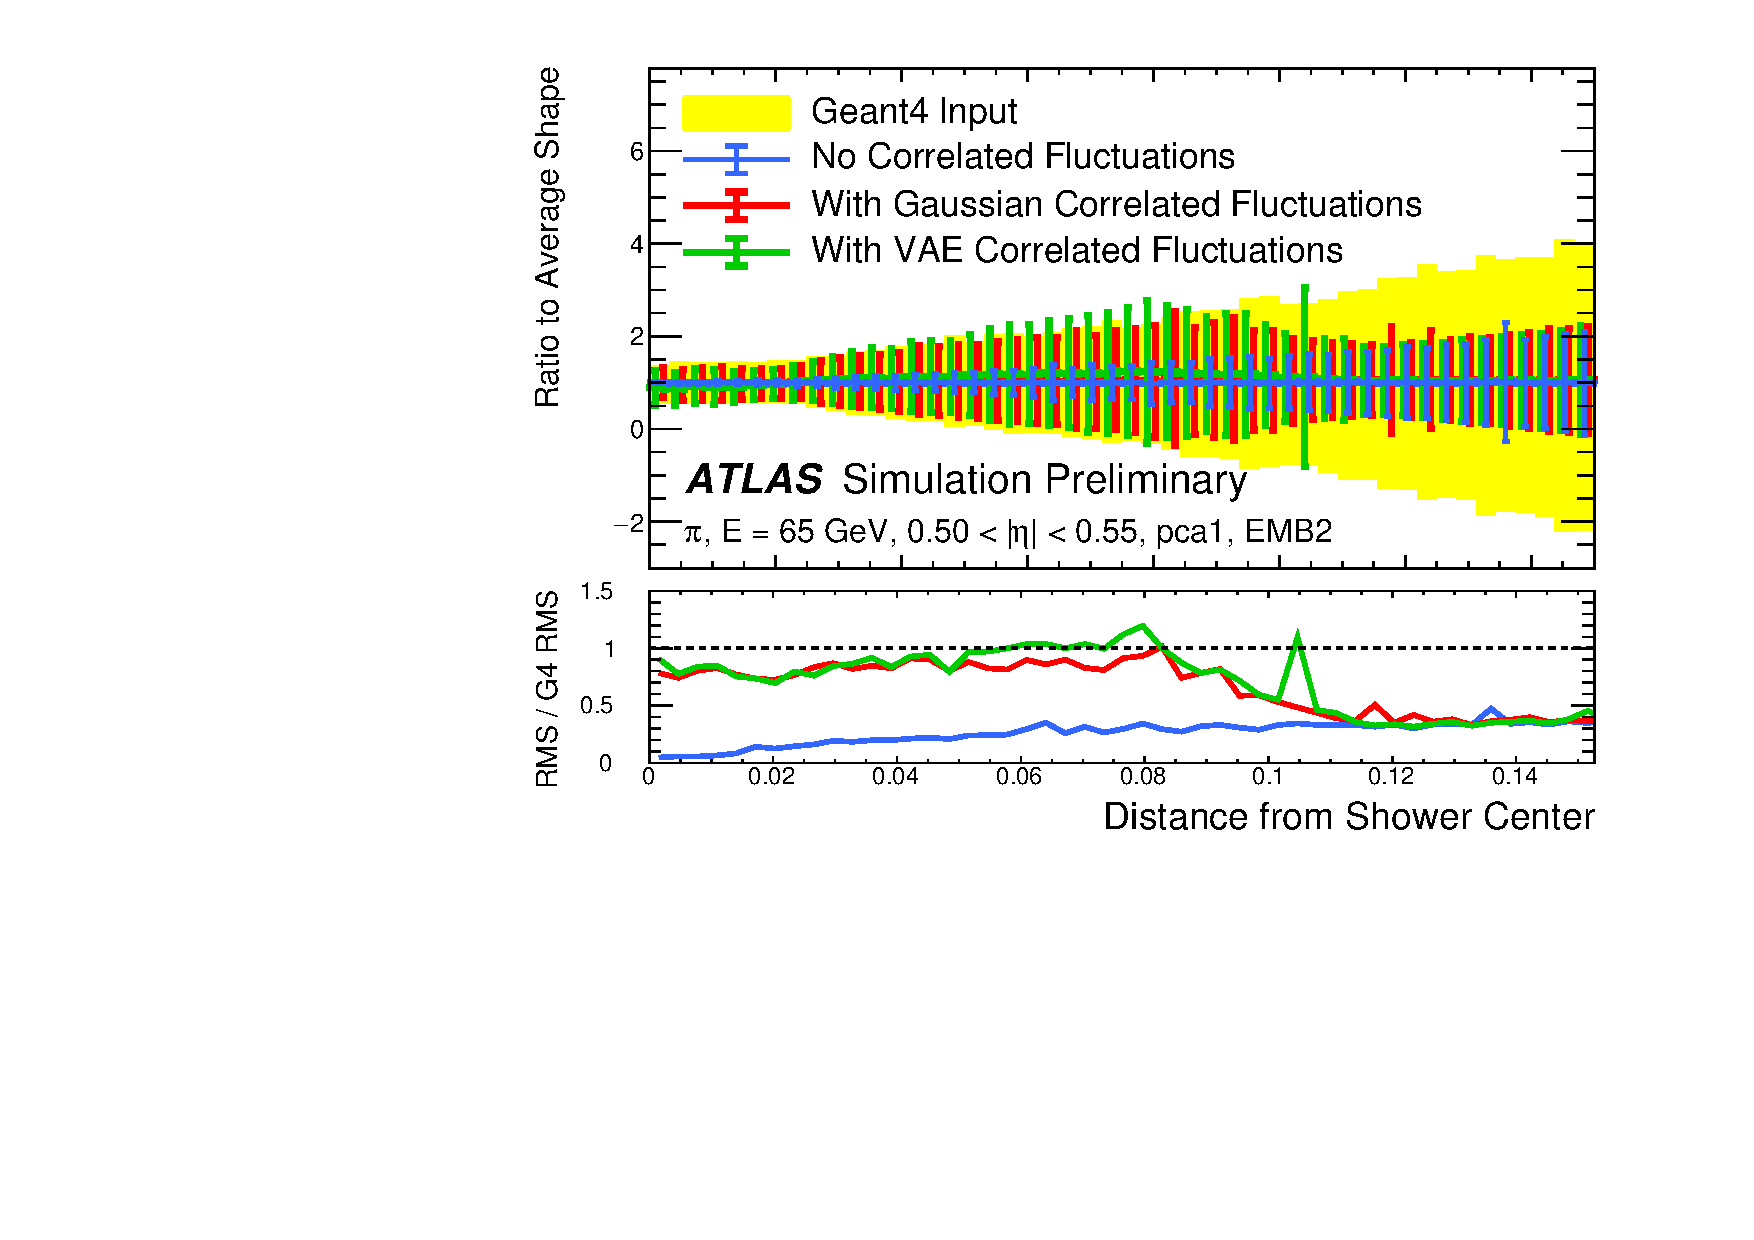
\includegraphics[width=0.48\textwidth]{figures/FCS-fig-05.pdf}
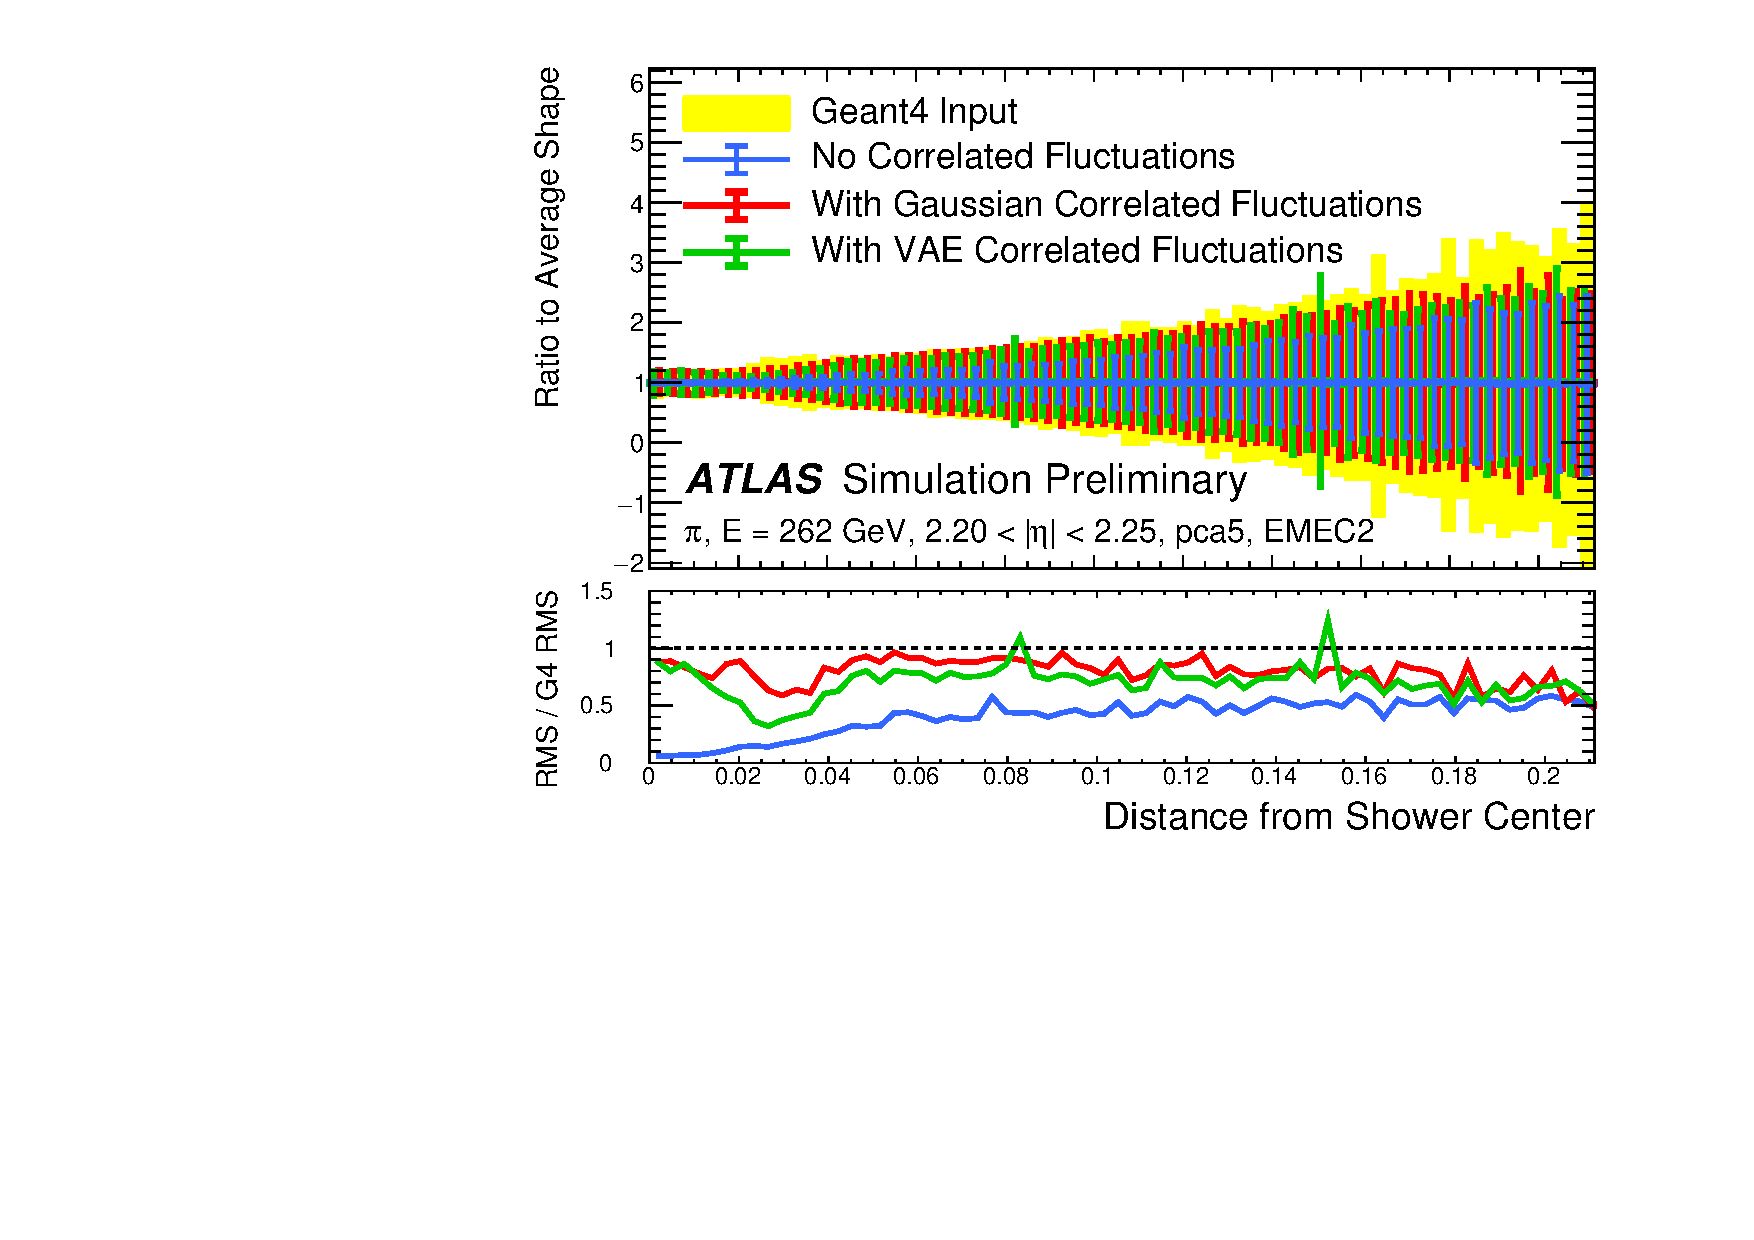
\includegraphics[width=0.48\textwidth]{figures/FCS-fig-06.pdf}
\caption{Comparison of the RMS fluctuations about the average shape with the Gaussian fluctuation model (red), the VAE fluctuation model (green), and without correlated fluctuations (blue) for a range of pion energies, $\eta$ points, and layers.}
\label{fig-5} 
\end{figure}

Validation of the Gaussian and VAE fluctuation methods was performed within FastCaloSimV2. Figure \ref{fig-5} shows the energy ratio of cells for a given simulation to the corresponding cells in the average shape as a function of the distance from the shower center. The mean for all simulation methods is expected to be around 1, with deviation from the average (the RMS fluctuation) shown by the error bars. The Gaussian method RMS (red) and VAE method RMS (green) both match the \GEANT RMS (yellow) better than the case without correlated fluctuations (blue) for a variety of energies, $\eta$ points, and layers, often reproducing $80 - 100\,\%$ of the \GEANT RMS magnitude, compared to the $5 - 30\,\%$ observed in the no correlated fluctuations case.

\begin{figure}[ht!]
\centering
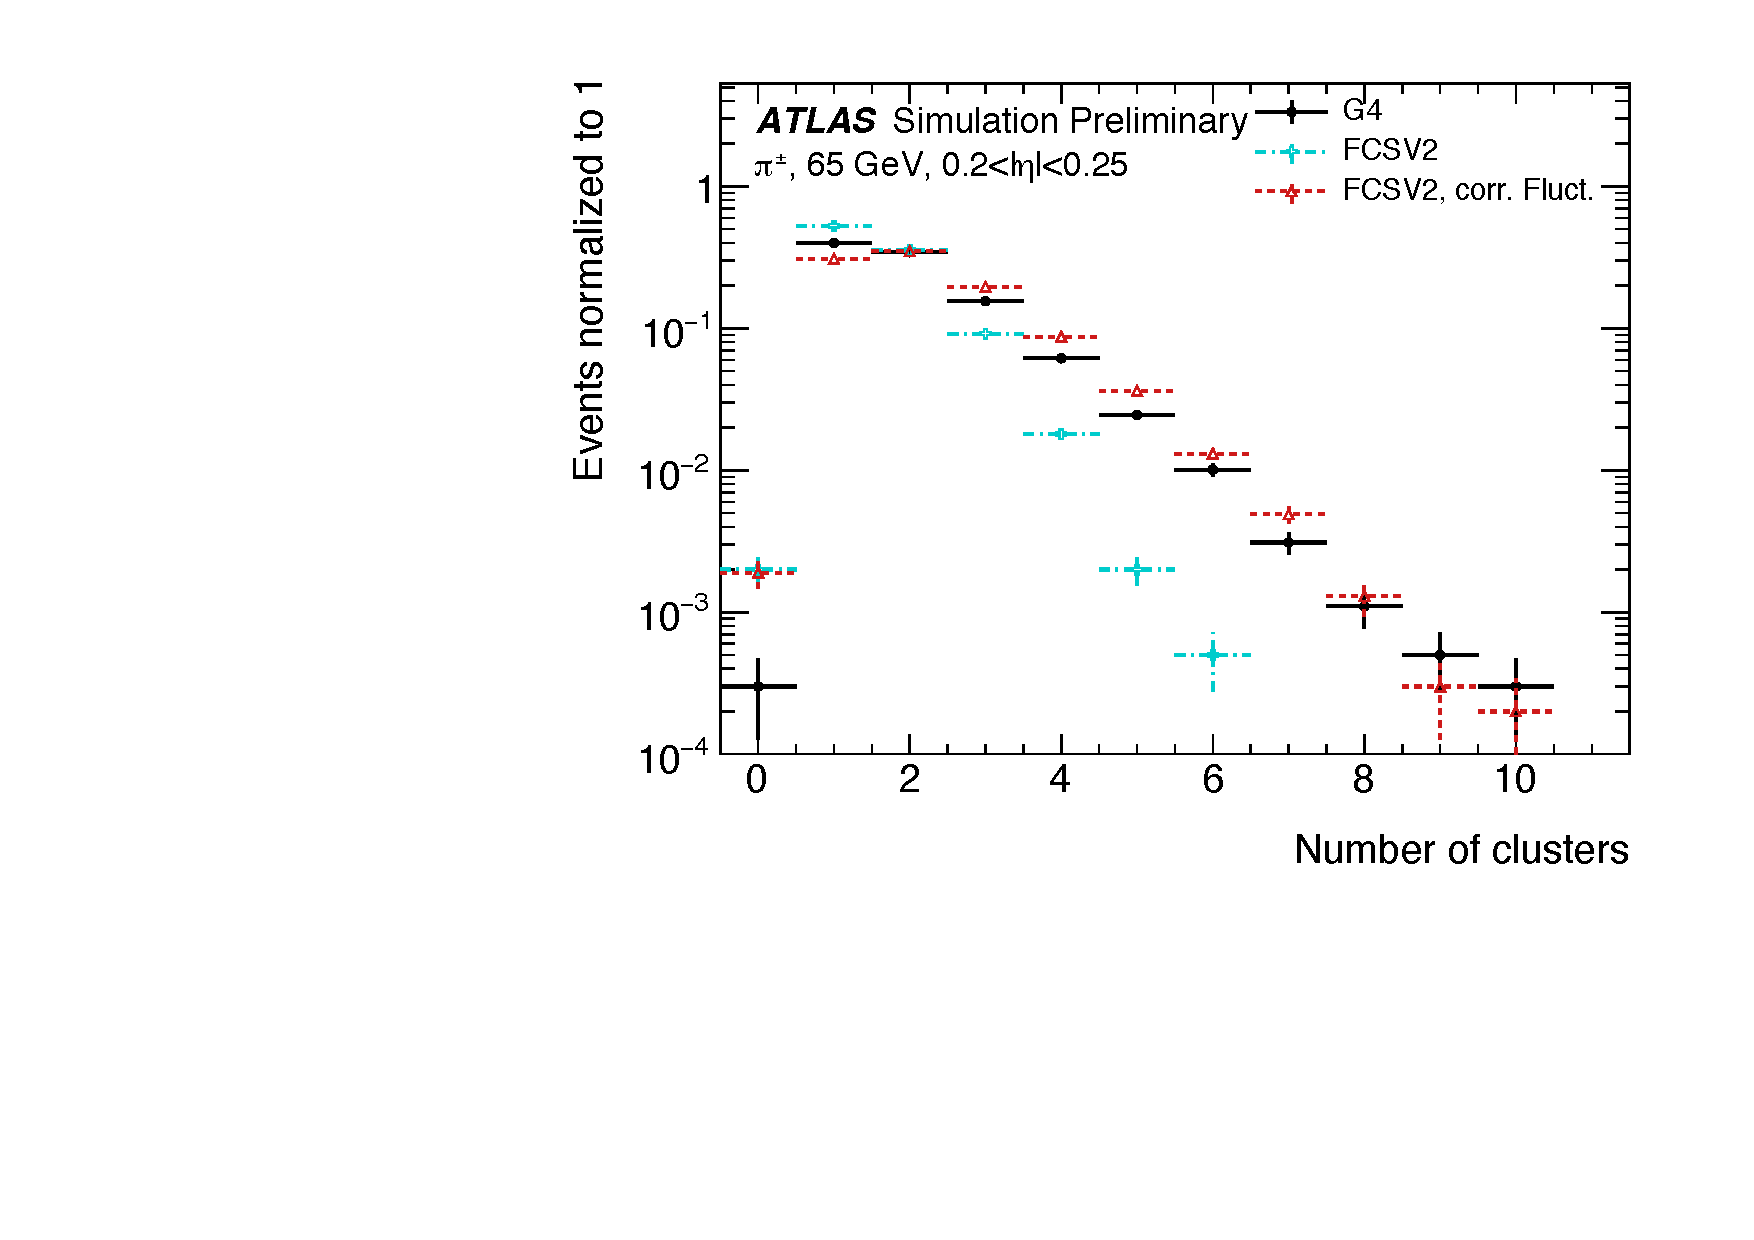
\includegraphics[width=0.48\textwidth]{figures/FCS-fig-07.pdf}
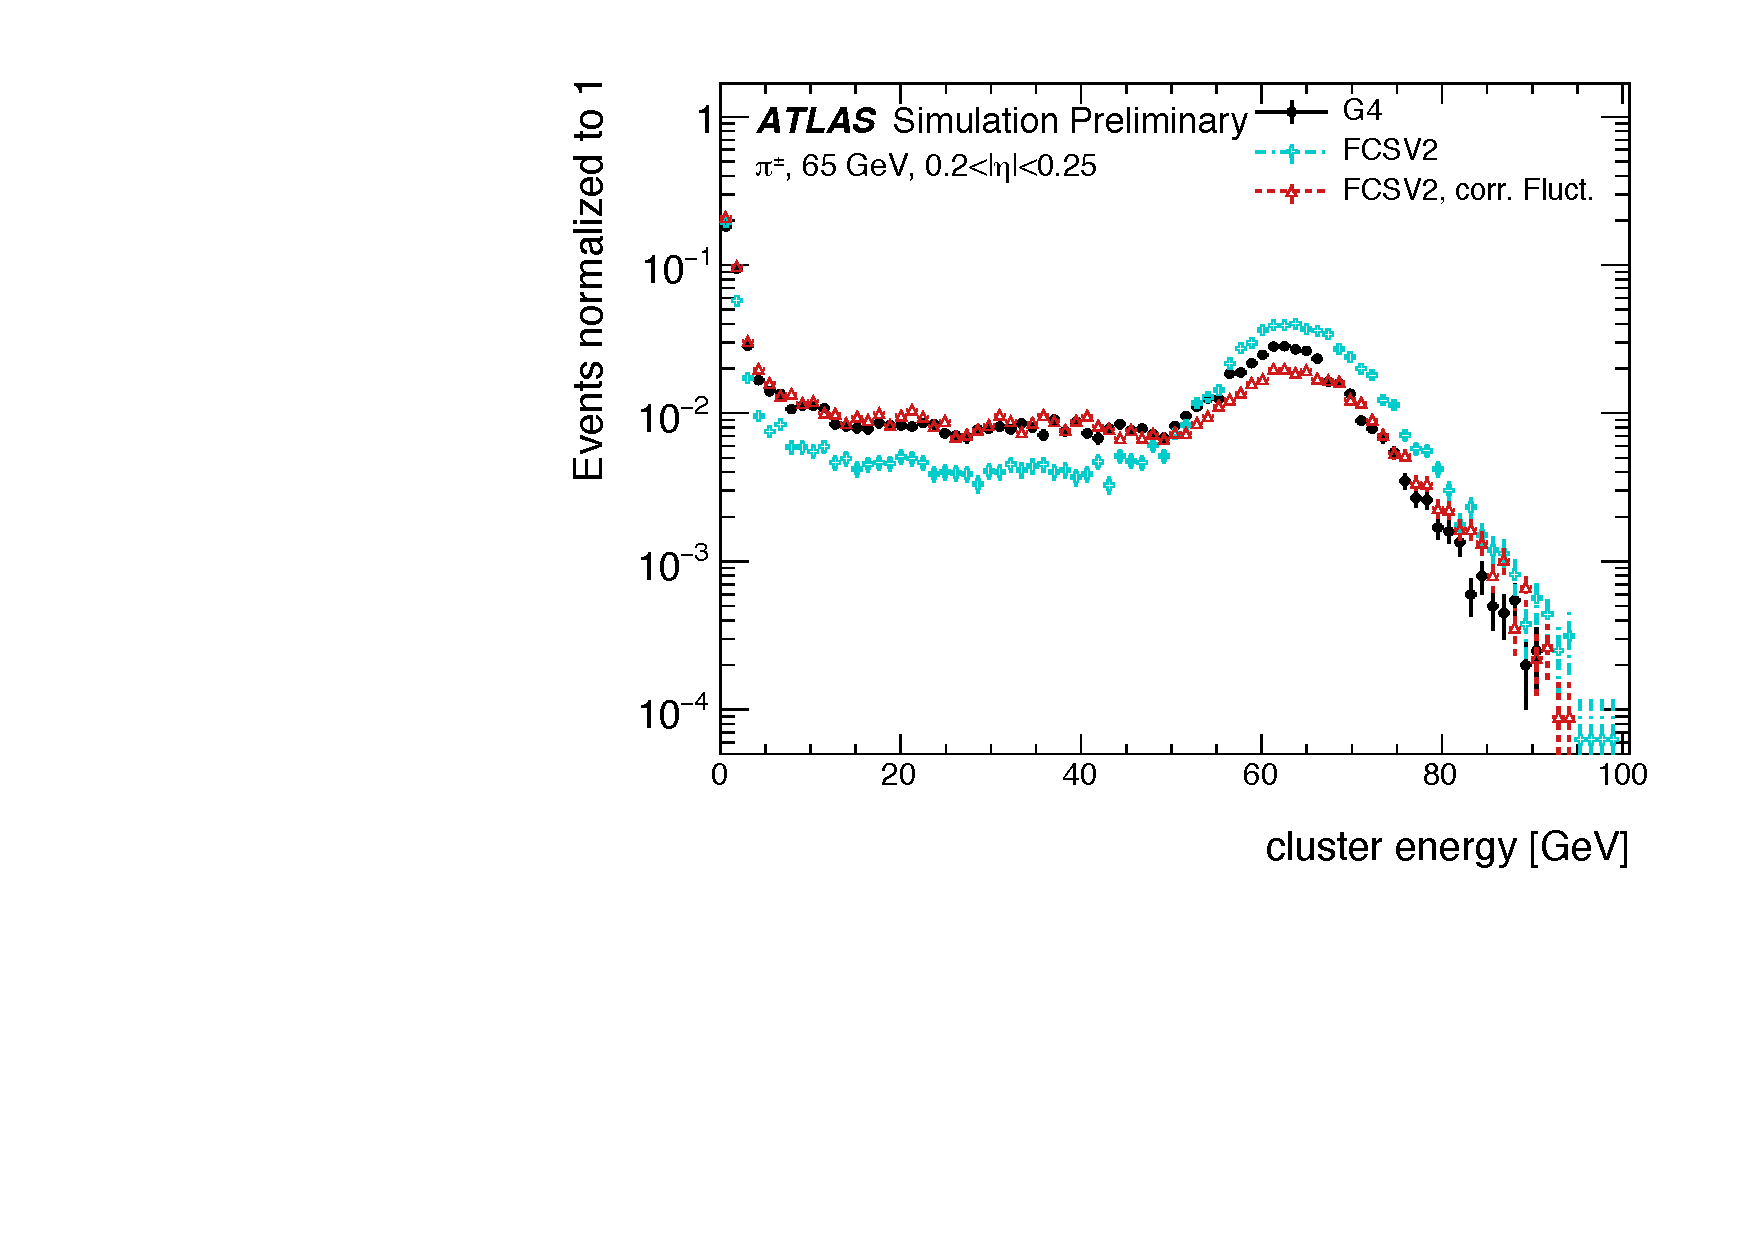
\includegraphics[width=0.48\textwidth]{figures/FCS-fig-08.pdf}
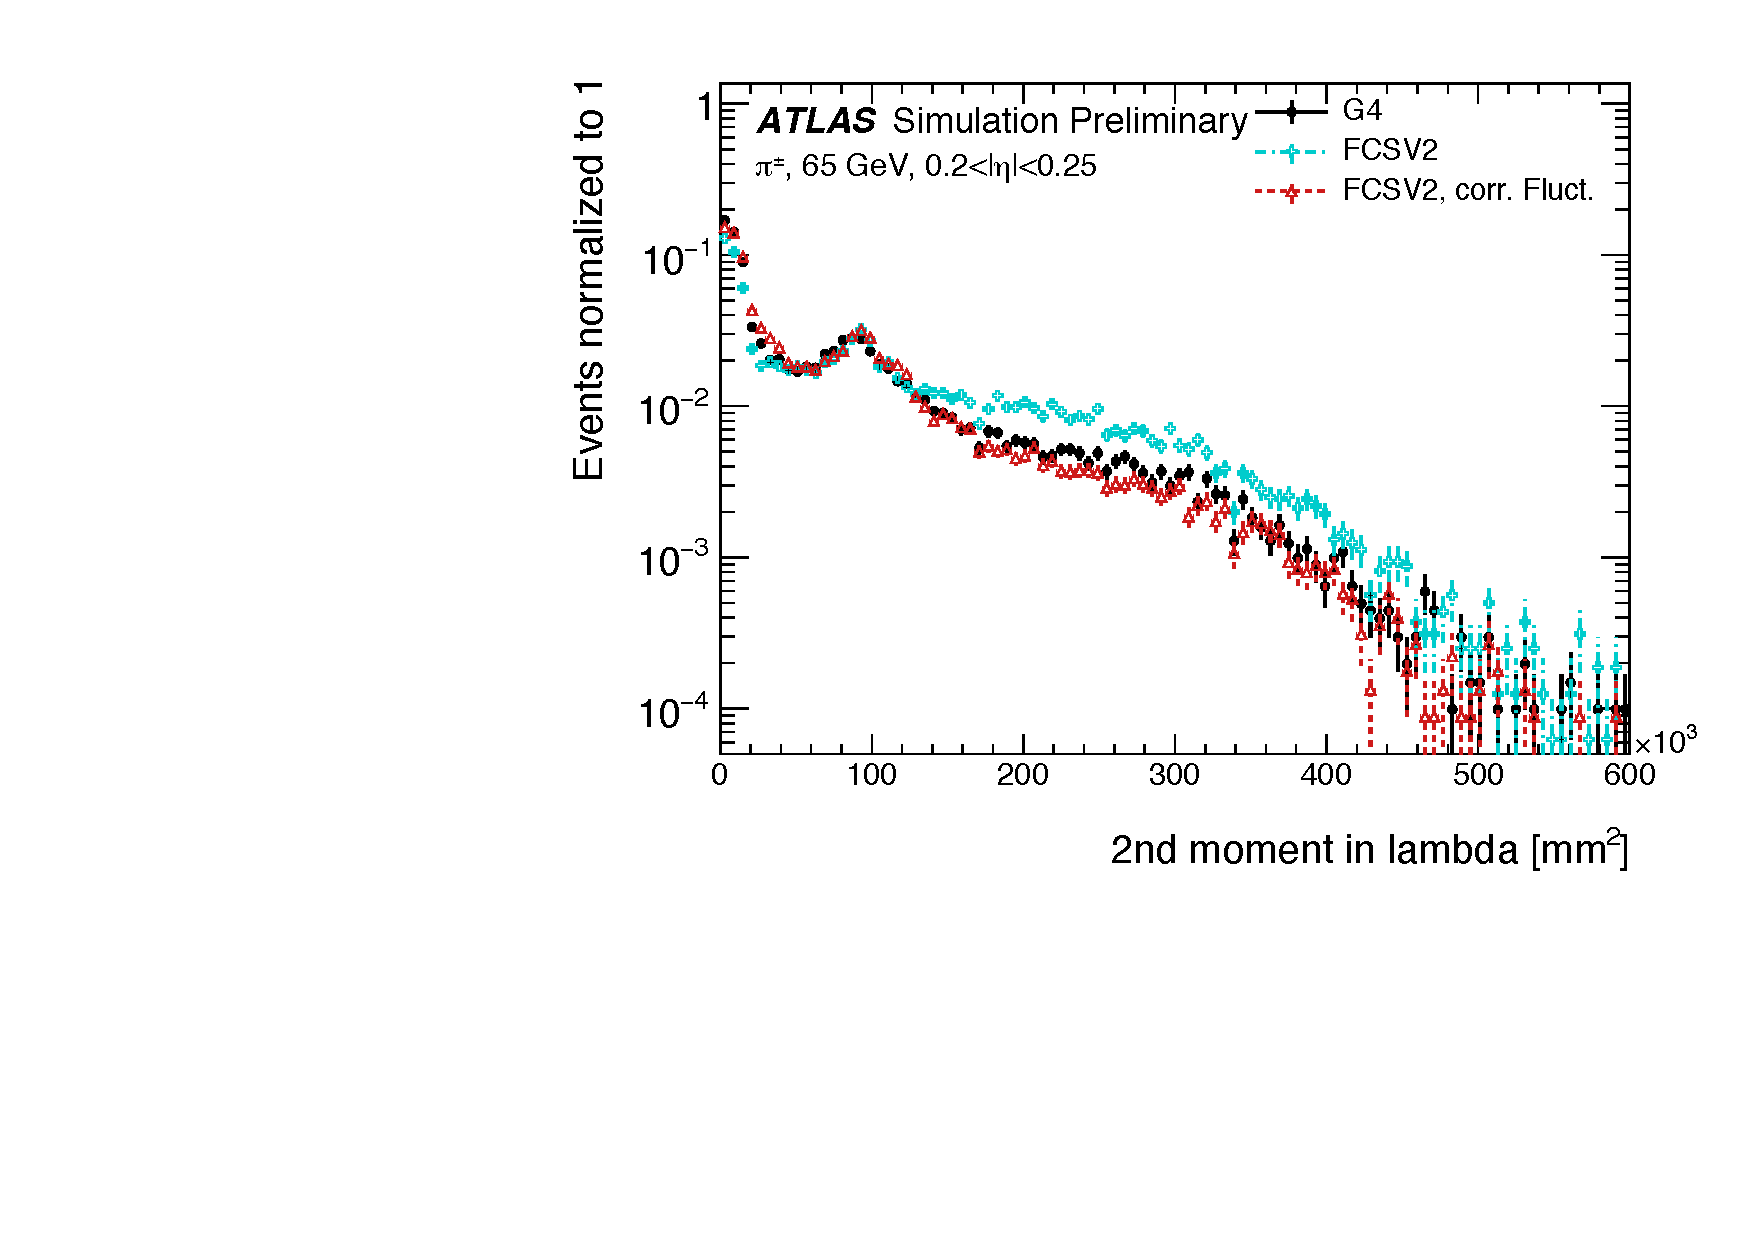
\includegraphics[width=0.48\textwidth]{figures/FCS-fig-10.pdf}
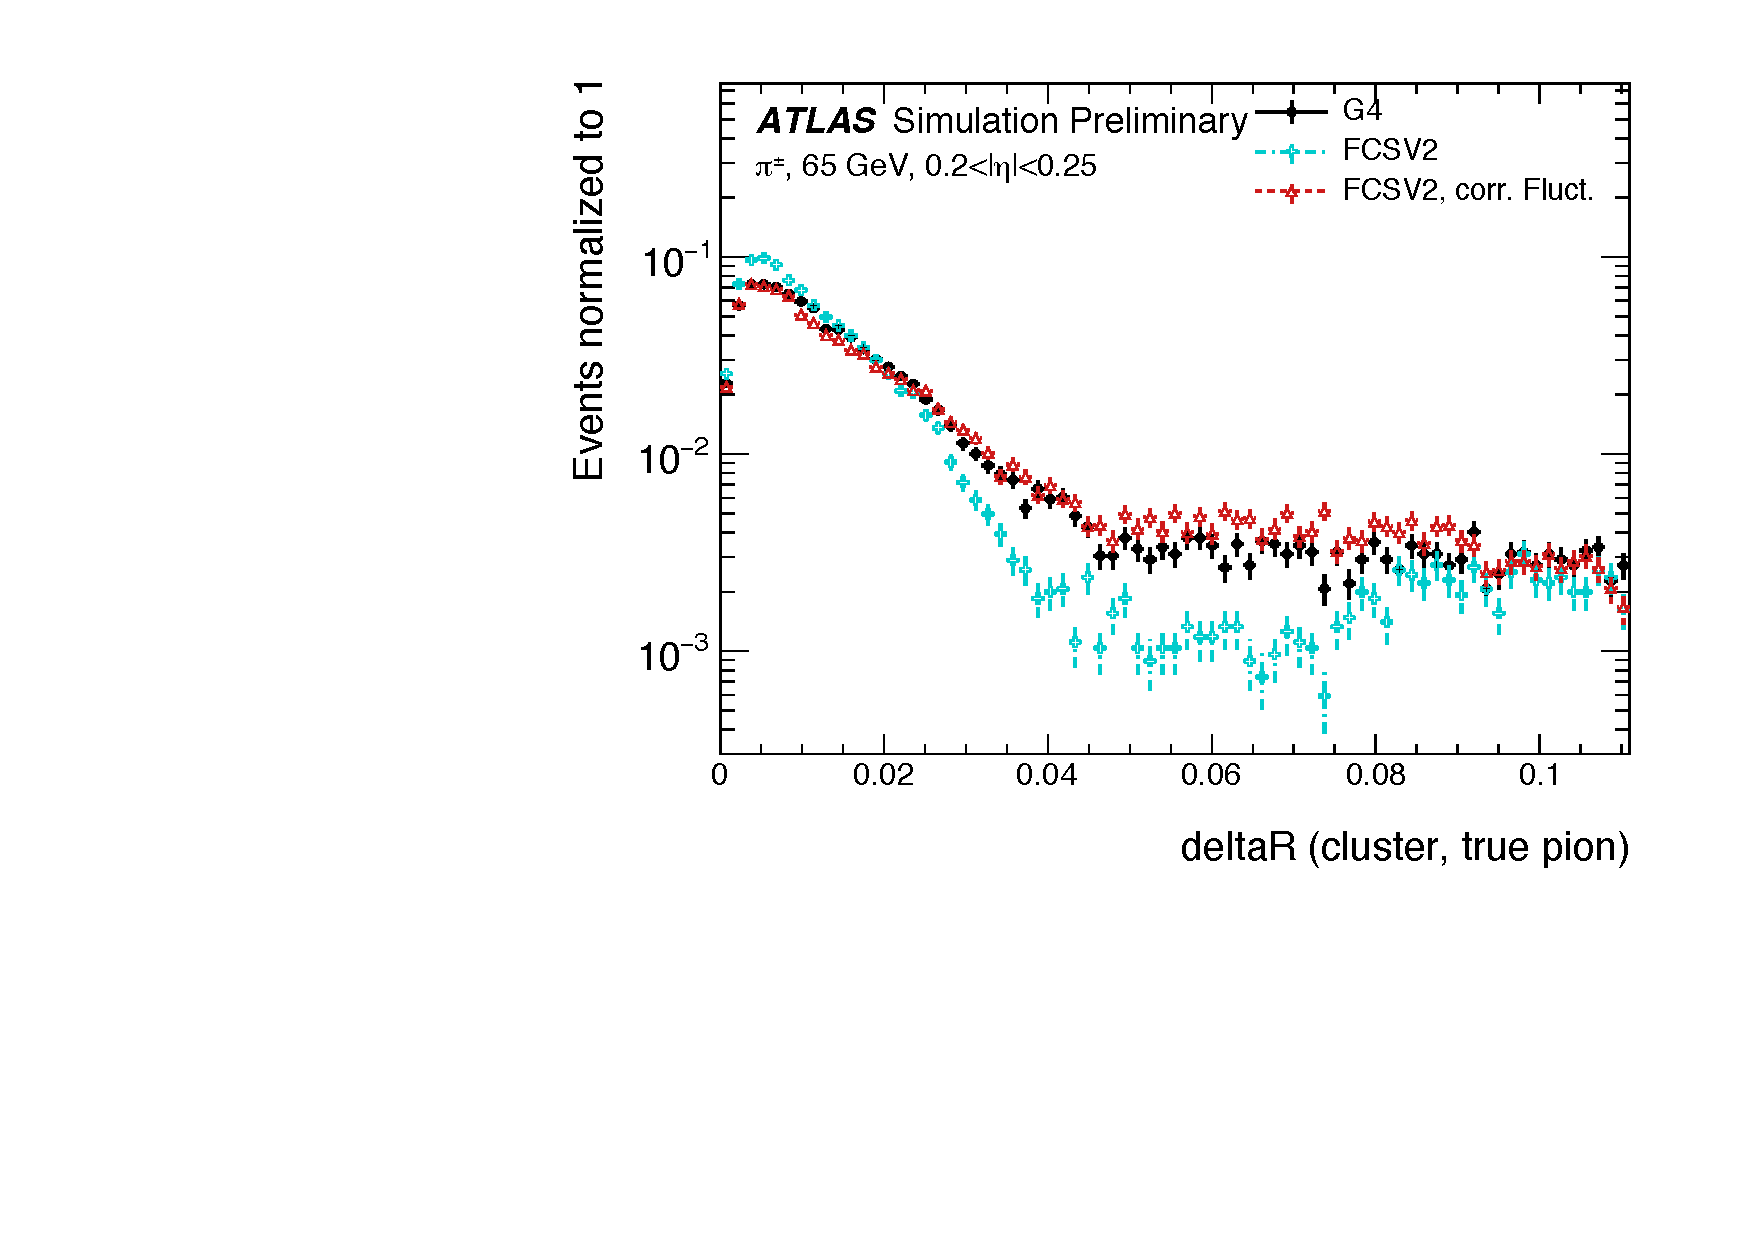
\includegraphics[width=0.48\textwidth]{figures/FCS-fig-11.pdf}
\caption{Comparison of the Gaussian fluctuation model to the default FCSV2 version and to G4 simulation, using pions of 65 GeV 
energy and $0.2 < |\eta| < 0.25$. Variables shown relate to calorimeter clusters, three-dimensional spatial groupings 
of cells~\cite{TopoCluster} which provide powerful insight on the structure of energy deposits in the calorimeter. 
Variables considered include number and energy of clusters, the 2nd moment in lambda, ($<\lambda^2>$), which 
describes the square of the longitudinal extension of a cluster, where $\lambda$ is the distance of a cell from the 
shower center along the shower axis, and a cluster moment is defined as $<x^n> =\frac{\sum E_{i}x_i}{\sum E_i}$, 
and the distance $\Delta R$, between the cluster and the true pion. With the correlated fluctuations, variables demonstrate 
improved modeling relative to default FastCaloSimV2.}
\label{fig-6} 
\end{figure}


Figure \ref{fig-6} shows the result of a simulation with full ATLAS reconstruction for 65 GeV central pions with 
the Gaussian fluctuation model. Here a \emph{cluster}~\cite{TopoCluster} is defined as a three-dimensional spatial 
grouping of calorimeter cells which are summed based on the input signals relative to their neighboring cells. 
The multiplicity, shape, and spatial distribution of such clusters provides a powerful insight on the structure of energy deposits 
in the calorimeter, and good performance in cluster variables is a promising step towards good performance in the 
modeling of jet substructure, as these clusters may themselves be summed to form jets (see Chapter \ref{chap:reconstruction}). 
The simulation with the Gaussian fluctuation model demonstrates improved modeling of several of these cluster variables 
relative to baseline FastCaloSimV2, reproducing the distributions of events simulated with \GEANT. These include number and 
energy of clusters, the 2nd moment in lambda, ($<\lambda^2>$), which describes the square of the longitudinal extension of a 
cluster, where $\lambda$ is the distance of a cell from the shower center along the shower axis, and a cluster moment is defined 
as $<x^n> =\frac{\sum E_{i}x_i}{\sum E_i}$, and the distance $\Delta R$, between the cluster and the true pion.

The new fast calorimeter simulation is a crucial part of the future of simulation for the ATLAS Experiment at the LHC. 
The per event simulation time of the full detector with \GEANT, calculated over 100 $t\bar{t}$ events, is 228.9 s. 
Using FastCaloSim for the calorimeter simulation reduces this to 26.6 s, of which FastCaloSim itself is only 0.015 s, 
with the majority of the remaining simulation time due to \GEANT.
Good physics modeling is achieved, and the correlated fluctuations method shows good proof of concept improvement for 
the modeling of hadronic showers.

\FloatBarrier
\section{Outlook}
There has been significant effort in the community to develop a set of fast simulation tools, with the use of machine 
learning methods at the forefront of such approaches (e.g. ~\cite{GAN-sim}, ~\cite{DijetGAN}). Most fast simulation approaches 
generally are based on parametrizations of fully simulated events, but fall into two paradigms - a ``by hand'' simulation, which 
focuses on the modeling of individual detector effects, or a fully parametrized simulation, 
in which a generative model (e.g. a Generative Adversarial Network or Variational Autoencoder) is trained to directly 
reproduce the input events. Both approaches can be extremely powerful, but each suffer from certain drawbacks. 
The ``by hand'' approach offers the advantage of direct encoding of expert knowledge -- if an effect needs to be modeled, 
a new parametrization is introduced. However, by the same token, it requires dedicated parametrizations for each effect. 
Fully parametrizing the simulation with a generative model offloads this burden onto the network itself. However, by doing so, 
the ability to use expert knowledge is diminished -- the network is required to learn all relevant effects.

The method presented here represents an effort to step towards a hybrid between these two approaches, leveraging the power of 
machine learning techniques for individual parametrizations within the by hand framework. Such hybrid solutions have the 
potential to be extremely powerful, and further work on the development of these solutions is an interesting direction of future study.

